\documentclass[11pt,a4paper]{article}

\usepackage[margin=1in]{geometry}
\usepackage{graphicx}
\usepackage{xcolor}
\usepackage{titlesec}
\usepackage{enumitem}
\usepackage{hyperref}
\usepackage{fancyhdr}
\usepackage{float}

\definecolor{brandpurple}{HTML}{6C63E8}
\definecolor{brandgray}{HTML}{4B4B57}

\titleformat{\section}{\normalfont\Large\bfseries\color{brandpurple}}{\thesection}{1em}{}
\titleformat{\subsection}{\normalfont\large\bfseries\color{brandgray}}{\thesubsection}{1em}{}

\pagestyle{fancy}
\fancyhf{}
\fancyhead[L]{MedRemind User Guide}
\fancyhead[R]{\thepage}
\renewcommand{\headrulewidth}{0.4pt}

\hypersetup{
    colorlinks=true,
    linkcolor=brandpurple,
    urlcolor=brandpurple,
}

\title{\textbf{\Huge MedRemind} \\[0.3em] \Large Your Smart Medicine Reminder \\[0.5em] \normalsize User Guide}
\author{}
\date{}

\begin{document}

\maketitle
\thispagestyle{empty}

\begin{center}
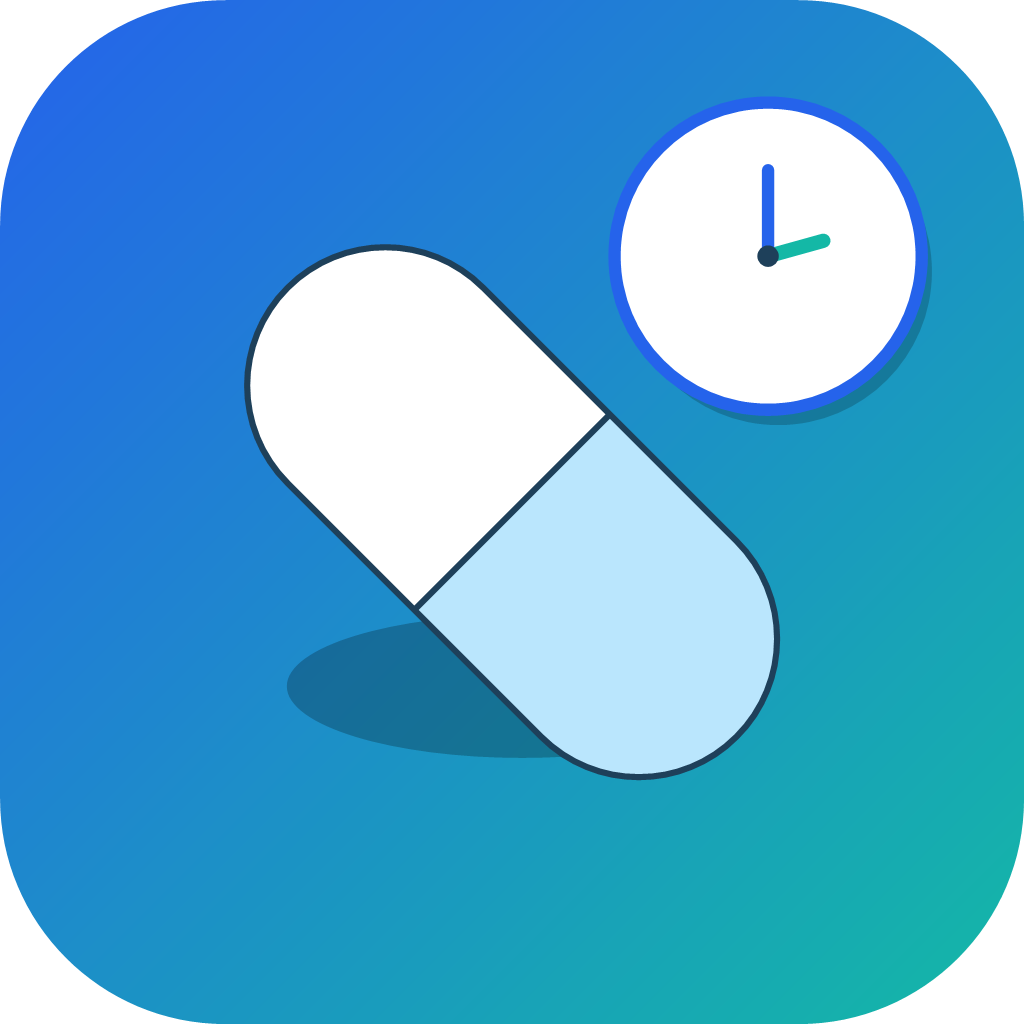
\includegraphics[width=0.3\textwidth]{screenshots/app_icon.png}
\end{center}

\newpage
\tableofcontents
\newpage

% ─────────────────────────────────────────────────────────────
\section{Introduction}

MedRemind is a smart medicine reminder app built for patients and caregivers
in Bangladesh. It helps you:

\begin{itemize}[leftmargin=1.5em]
    \item Keep a digital \textbf{Medicine Cabinet} of everything you take.
    \item Organize doses into \textbf{Dose Groups} (Morning, Afternoon,
        Evening, Night) with exact alarm times.
    \item Get a \textbf{full-screen alarm} that rings even when your phone
        screen is off or you're using another app.
    \item Track your \textbf{adherence} over time with a daily planner and
        a colour-coded history heatmap.
\end{itemize}

The app is subscribed to via your mobile operator's billing (Robi/Airtel,
through BDApps) at a small daily rate, and authenticates you with your phone
number and a password you choose.

% ─────────────────────────────────────────────────────────────
\section{Getting Started}

\subsection{Subscribe and Sign In}

When you first open MedRemind, you're shown the subscription screen, which
explains the price and the three headline features.

\begin{figure}[H]
    \centering
    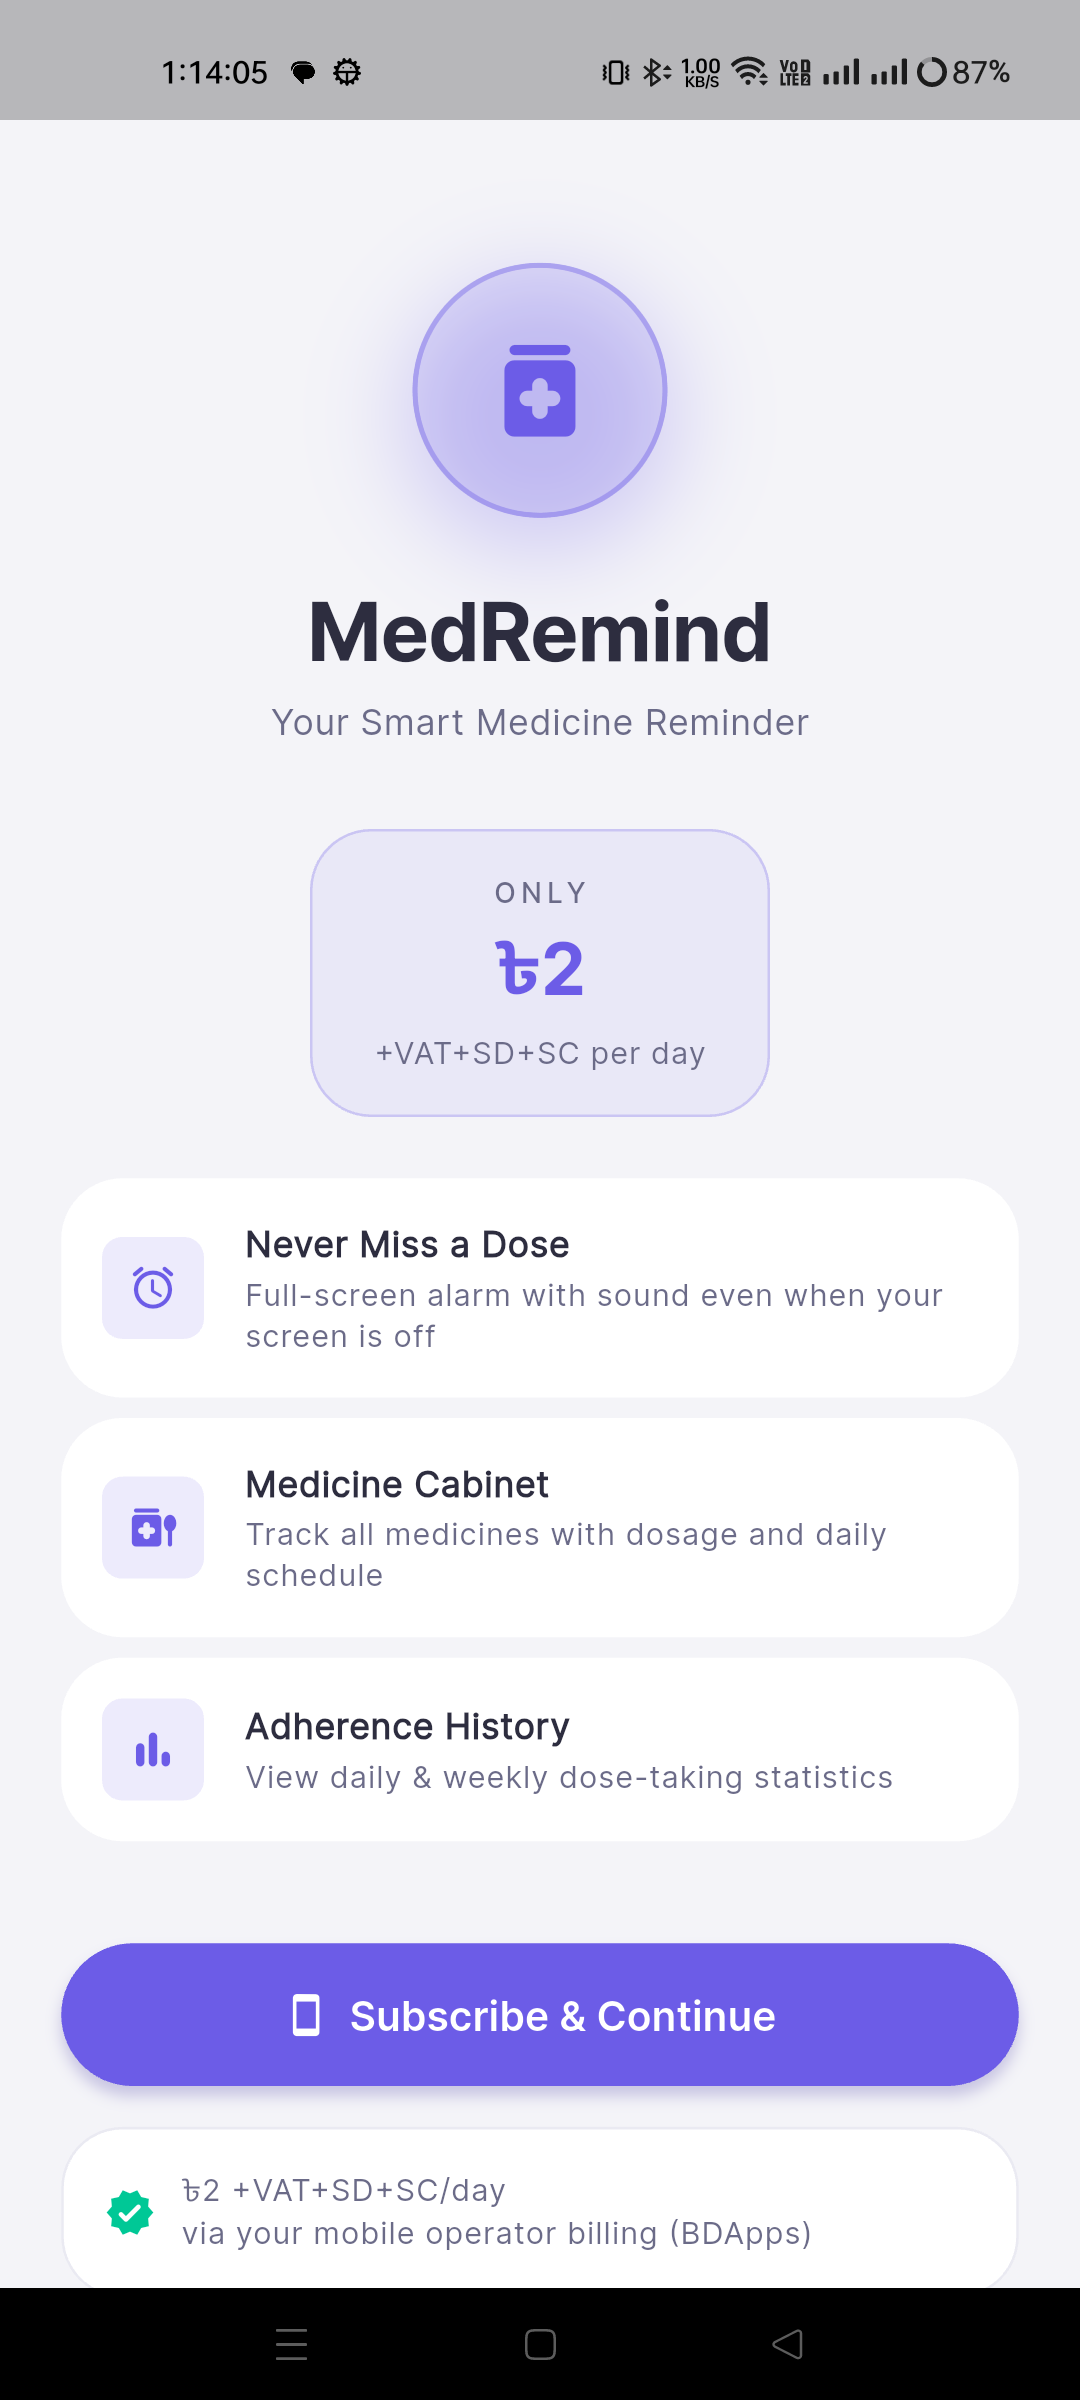
\includegraphics[width=0.45\textwidth]{screenshots/01_paywall.png}
    \caption{Subscription / welcome screen}
\end{figure}

Tapping \textbf{Subscribe \& Continue} takes you to the sign-in screen, where
you enter your mobile number. If the number is new, you'll be taken to
registration; if it already has an account, you'll be asked for your
password instead.

\begin{figure}[H]
    \centering
    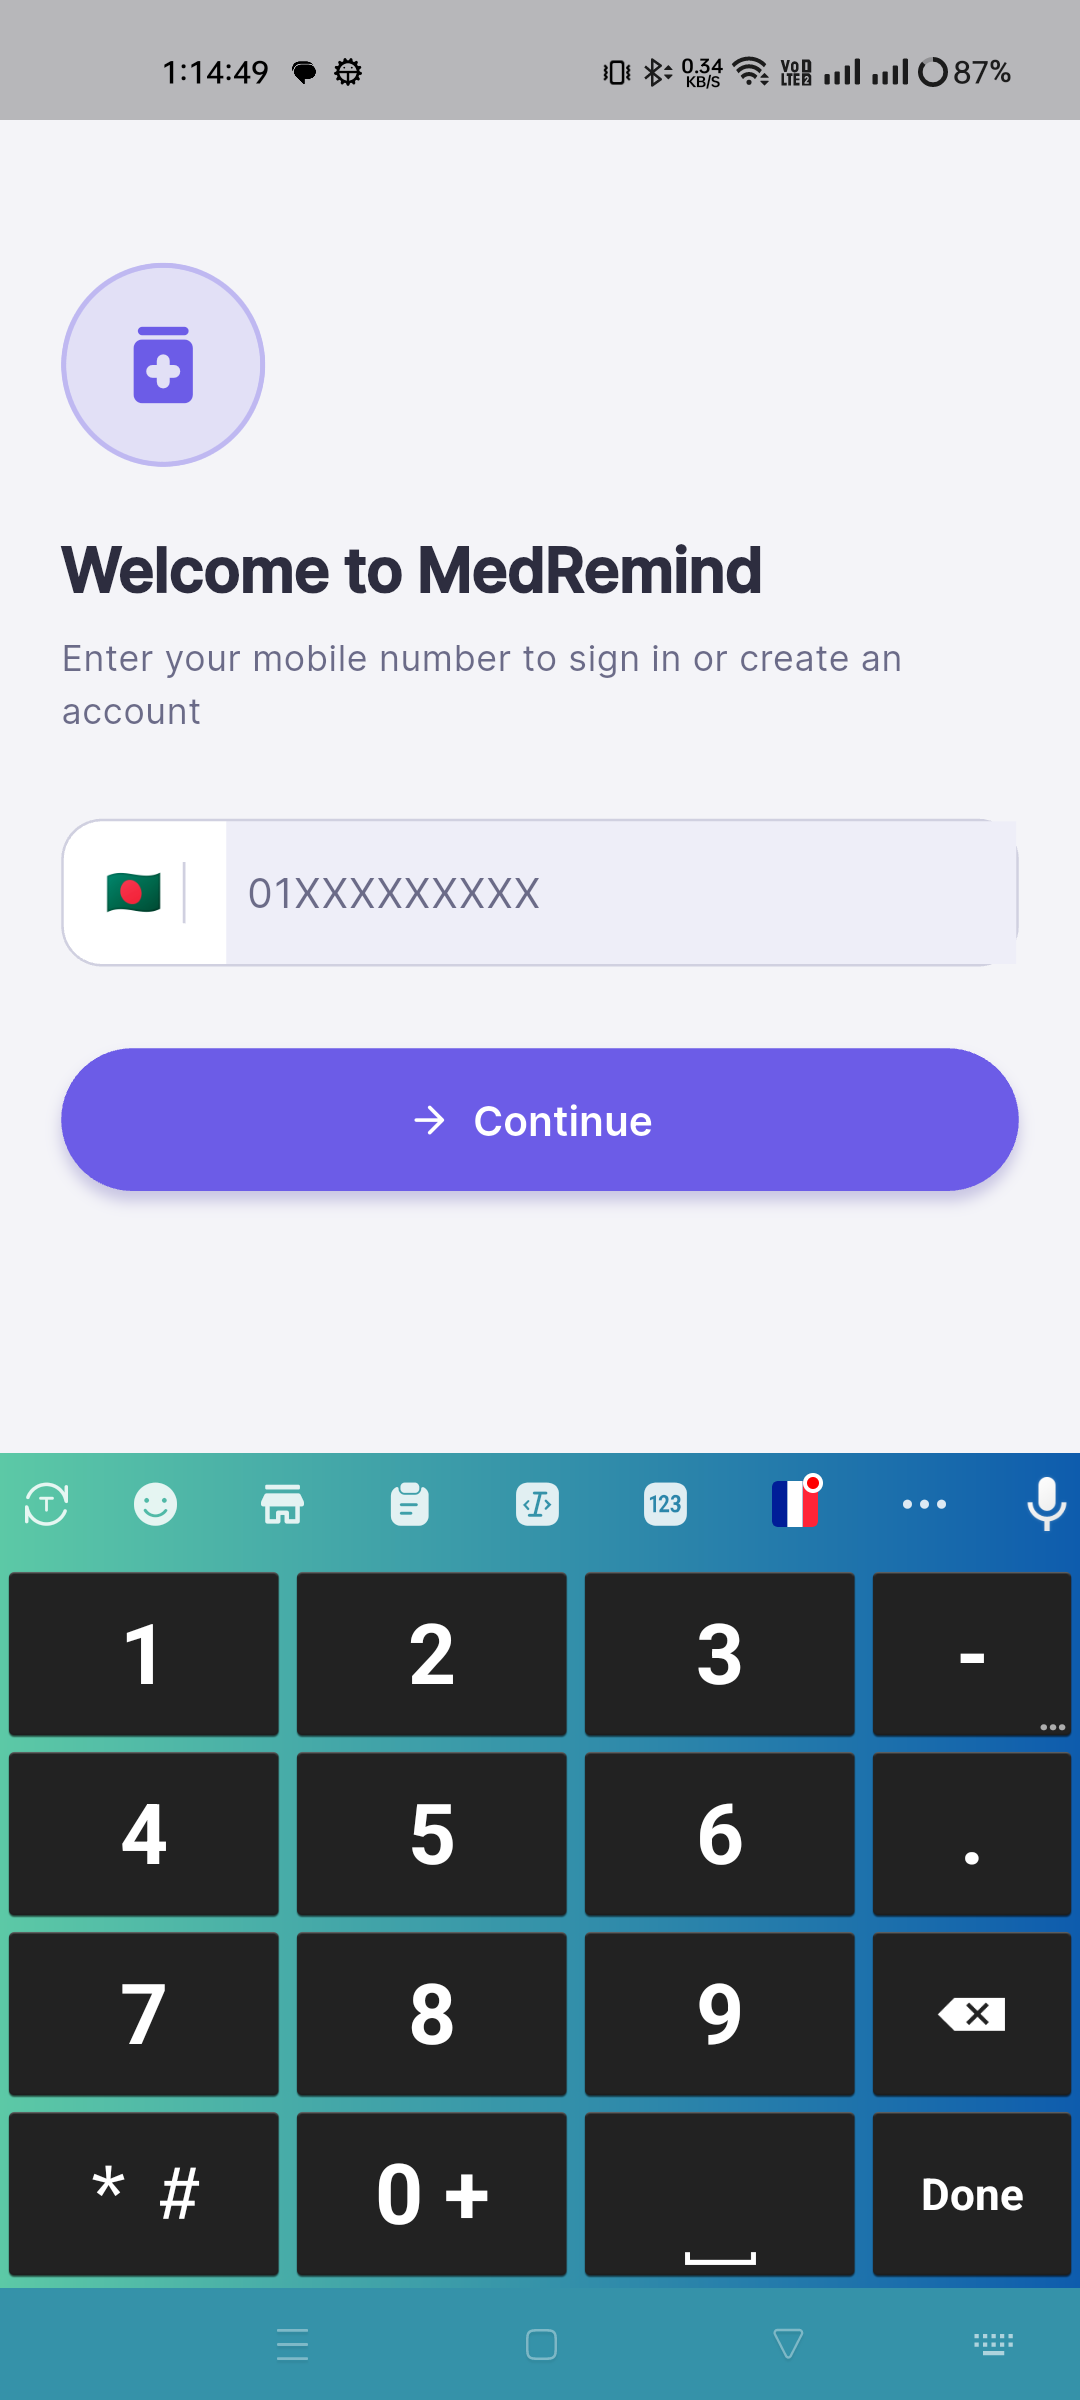
\includegraphics[width=0.45\textwidth]{screenshots/02_phone_entry.png}
    \caption{Enter your mobile number to sign in or register}
\end{figure}

\subsection{Create Your Account}

New numbers are asked for a name and a password (minimum 6 characters).

\begin{figure}[H]
    \centering
    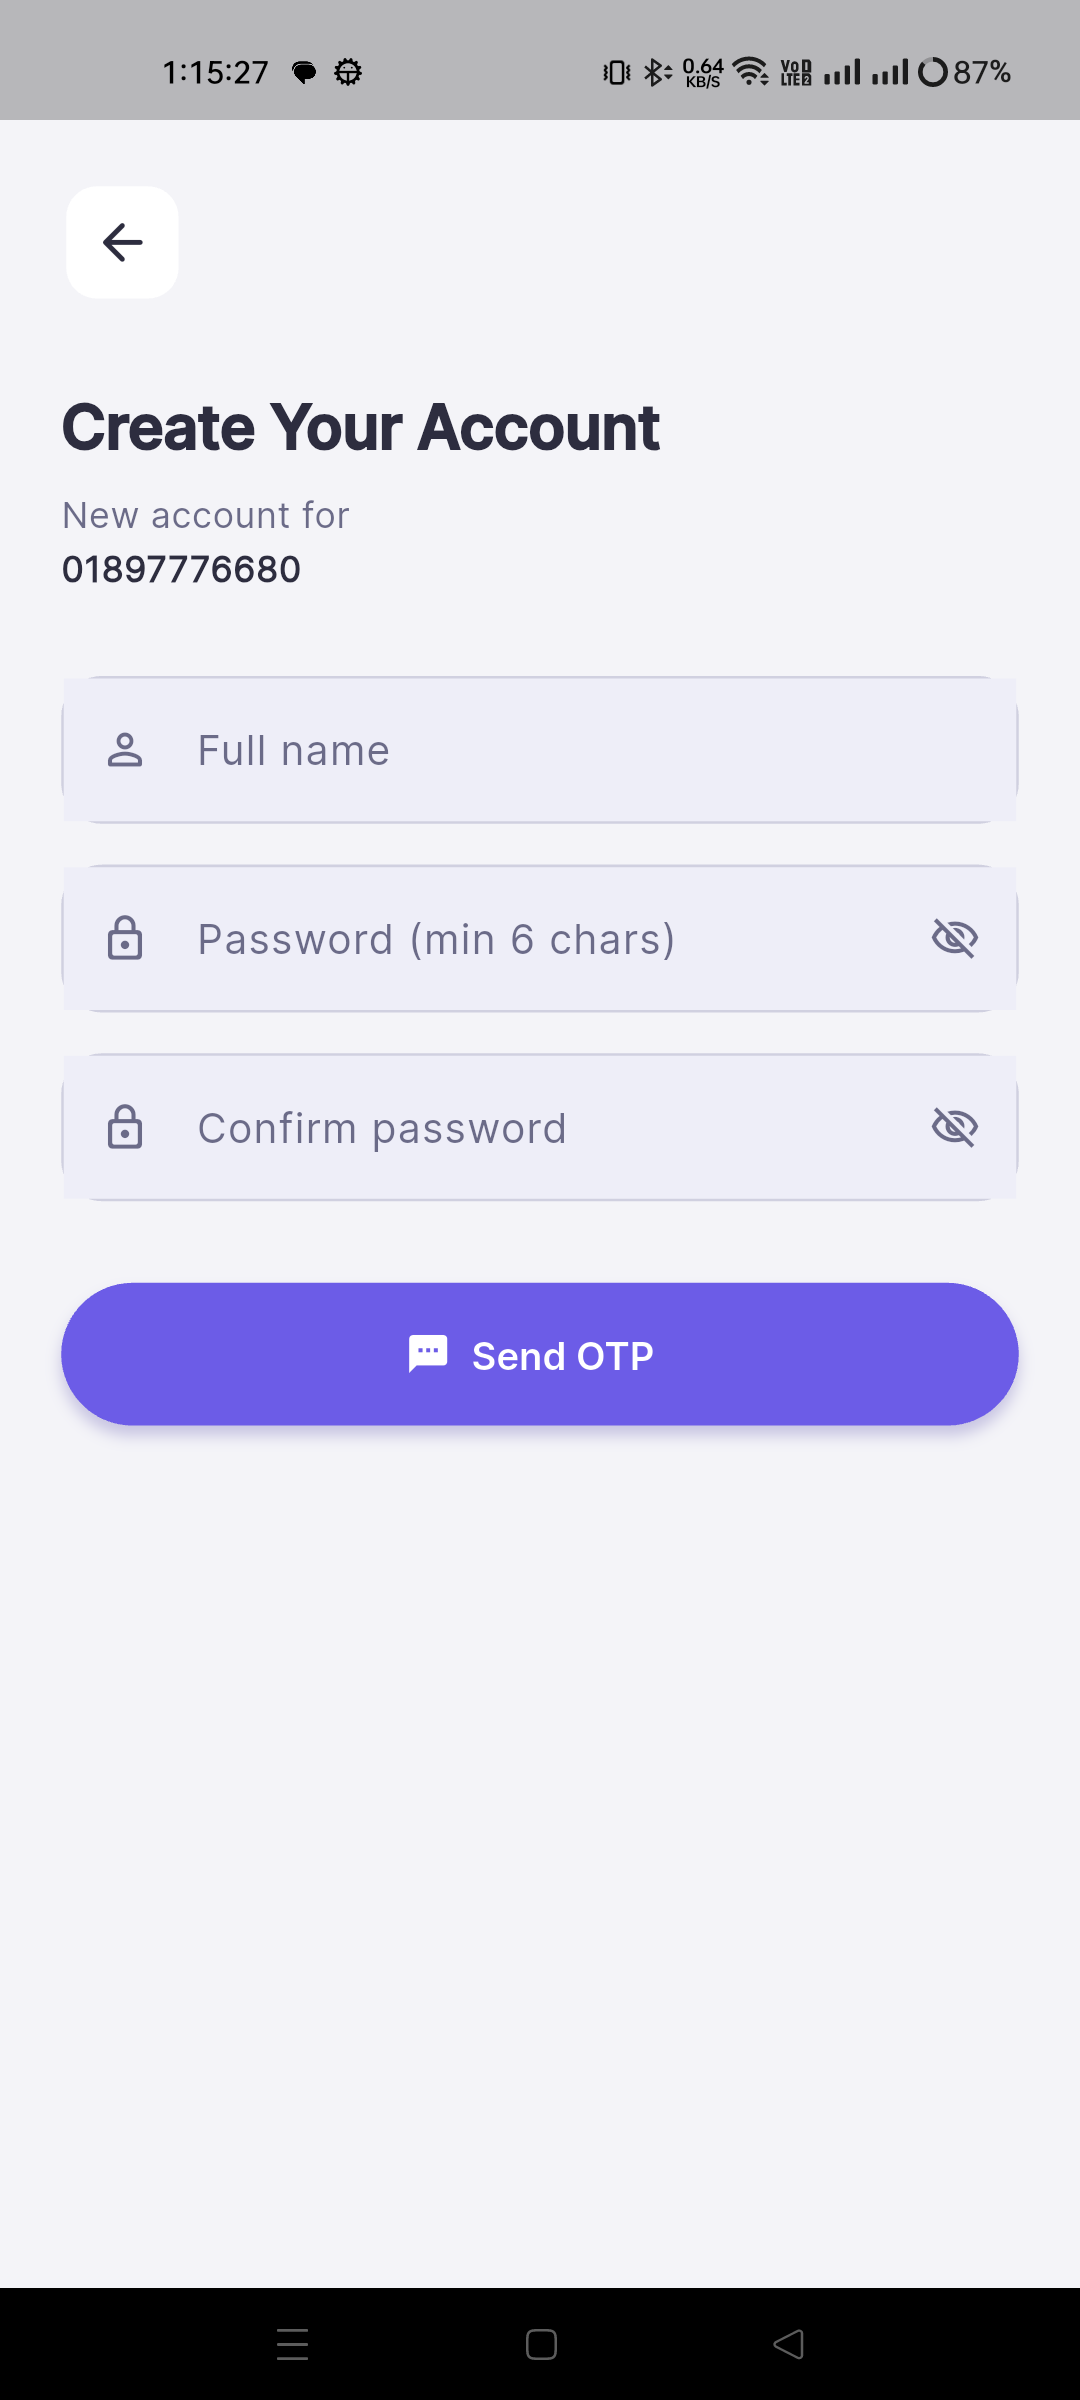
\includegraphics[width=0.45\textwidth]{screenshots/03_register.png}
    \caption{Create Your Account}
\end{figure}

After submitting, MedRemind sends a one-time SMS code to verify you own the
number before your account is created. Enter the 6-digit code on the OTP
screen to finish registration.

\subsection{Permission Onboarding}

A short three-screen walkthrough introduces the app's core value before you
grant any permissions:

\begin{figure}[H]
    \centering
    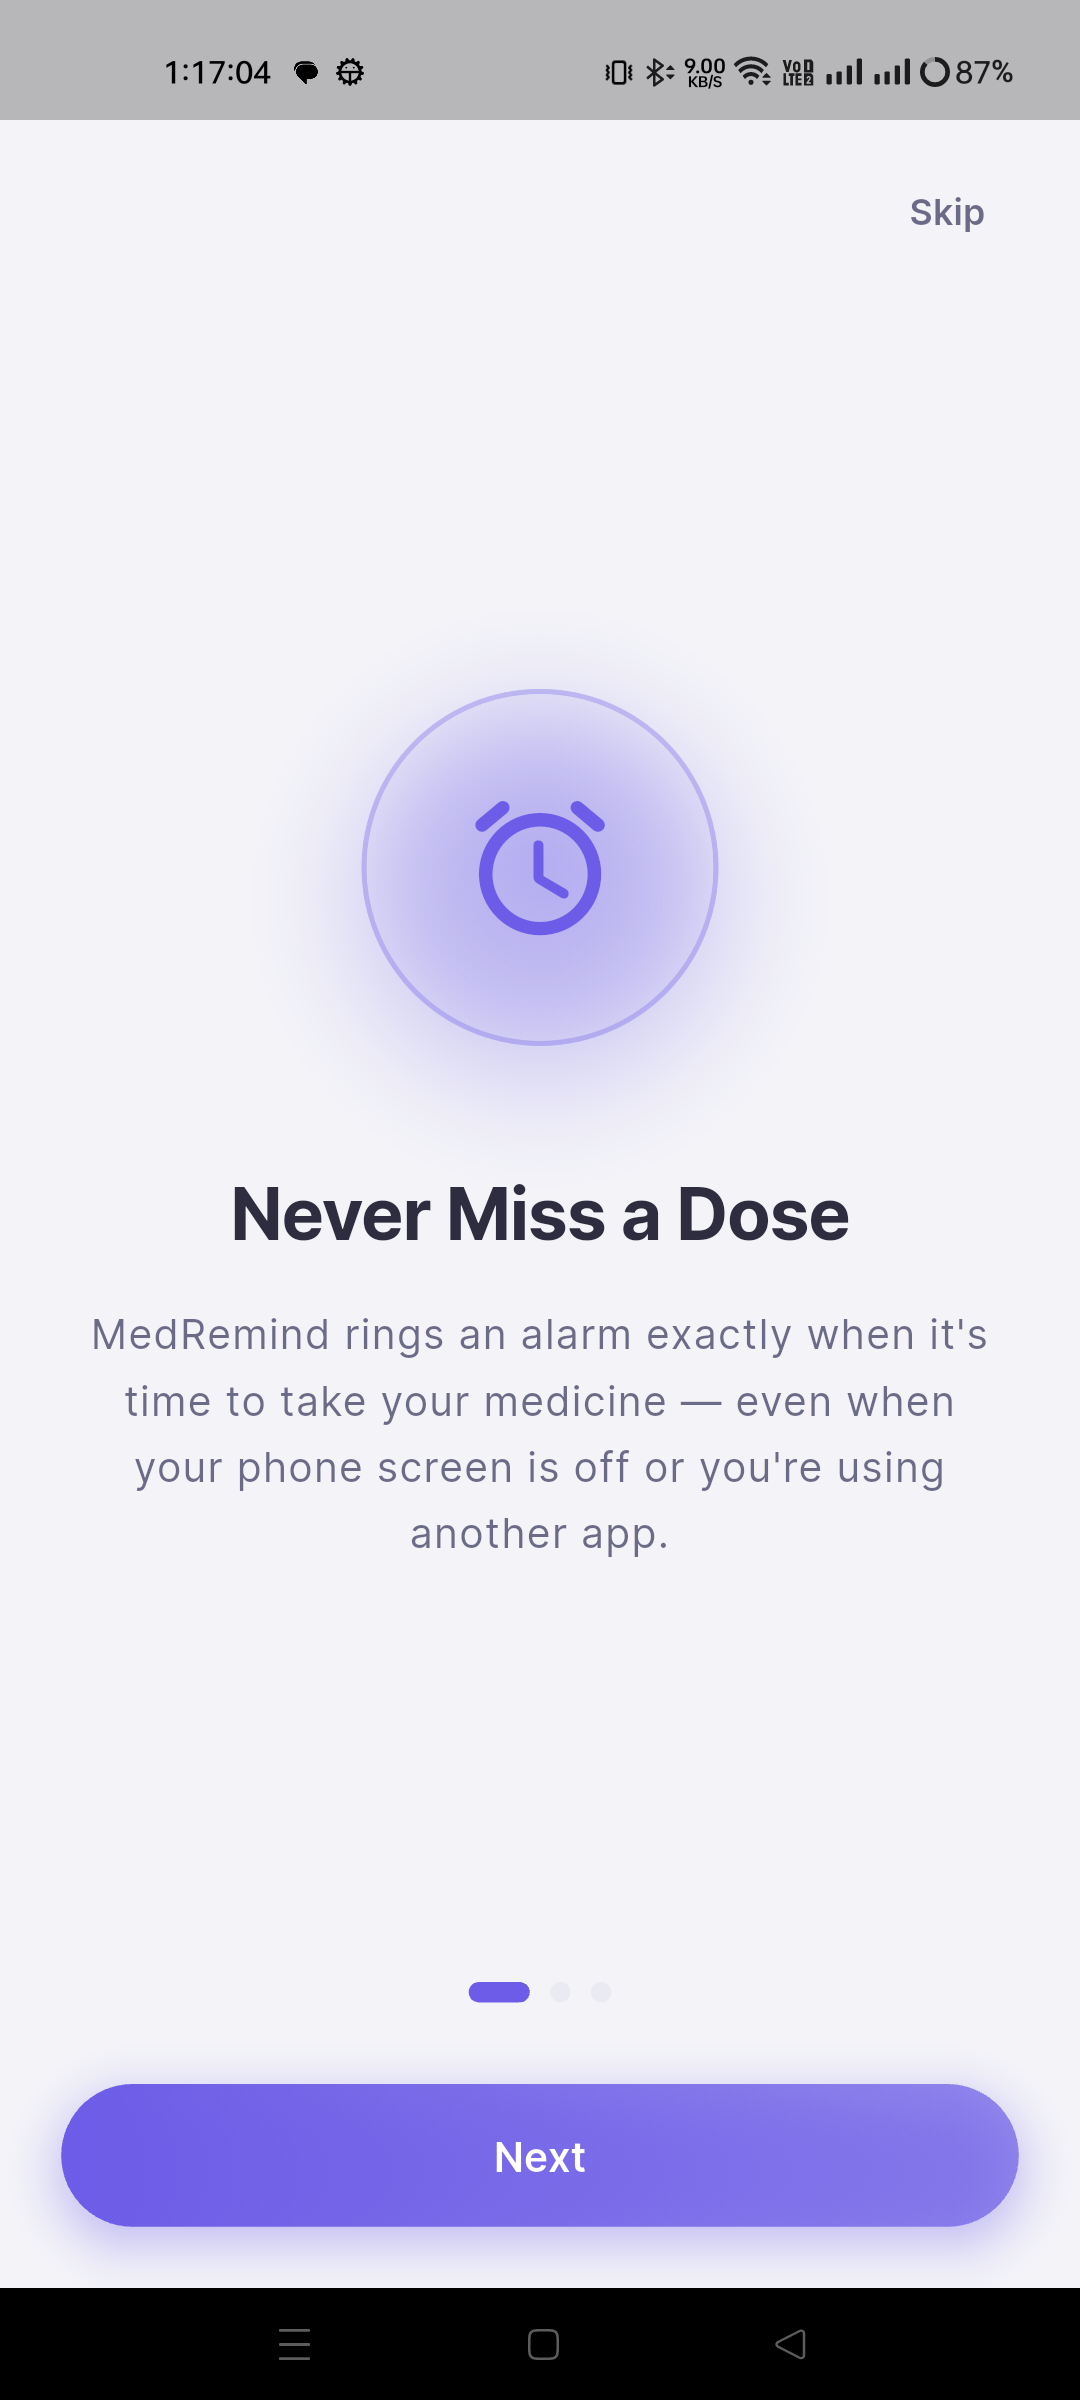
\includegraphics[width=0.32\textwidth]{screenshots/04_onboarding_1.png}\hfill
    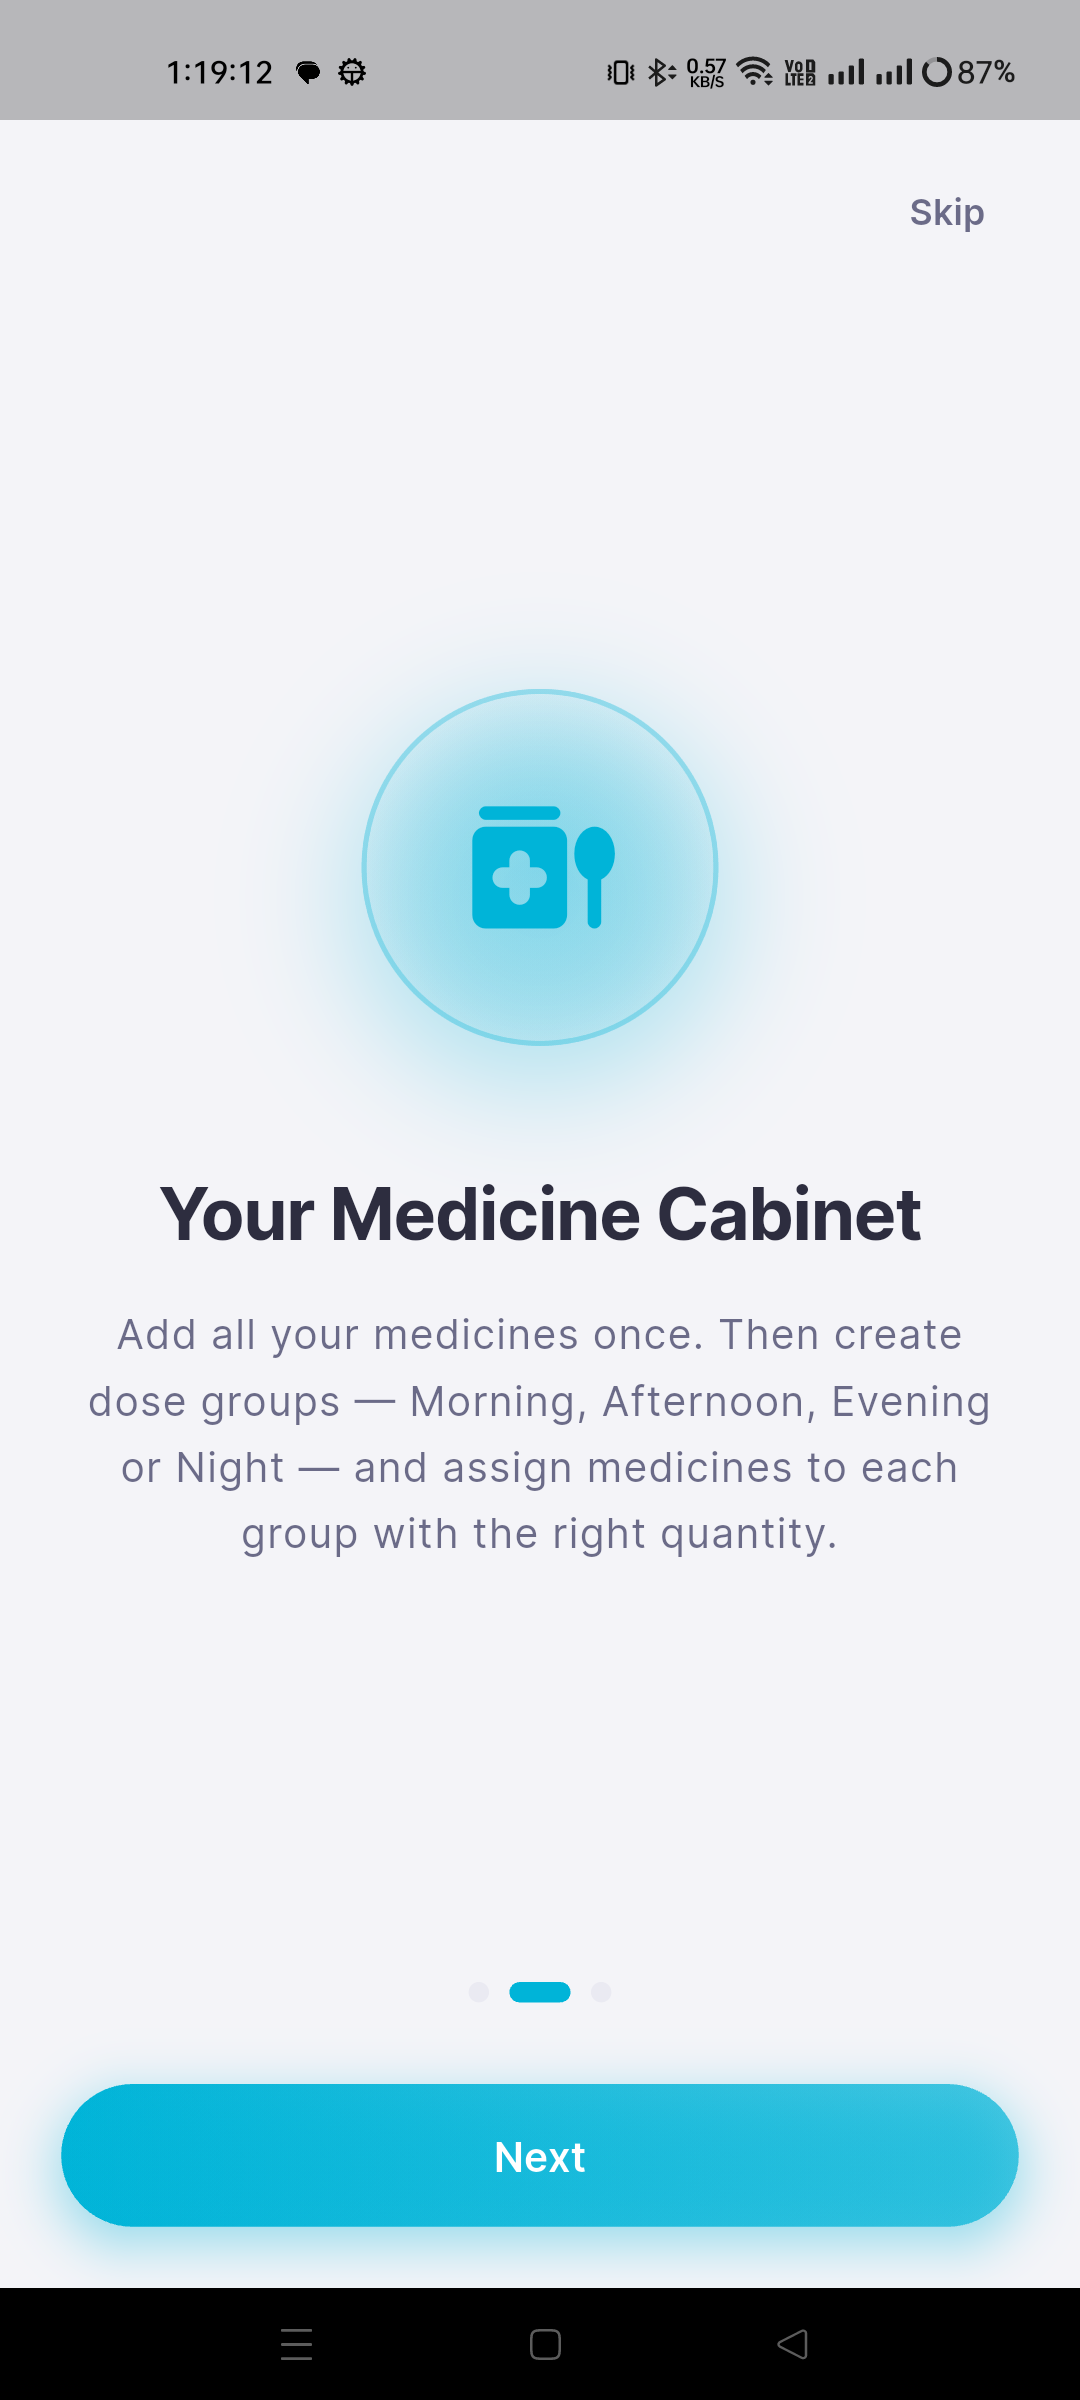
\includegraphics[width=0.32\textwidth]{screenshots/05_onboarding_2.png}\hfill
    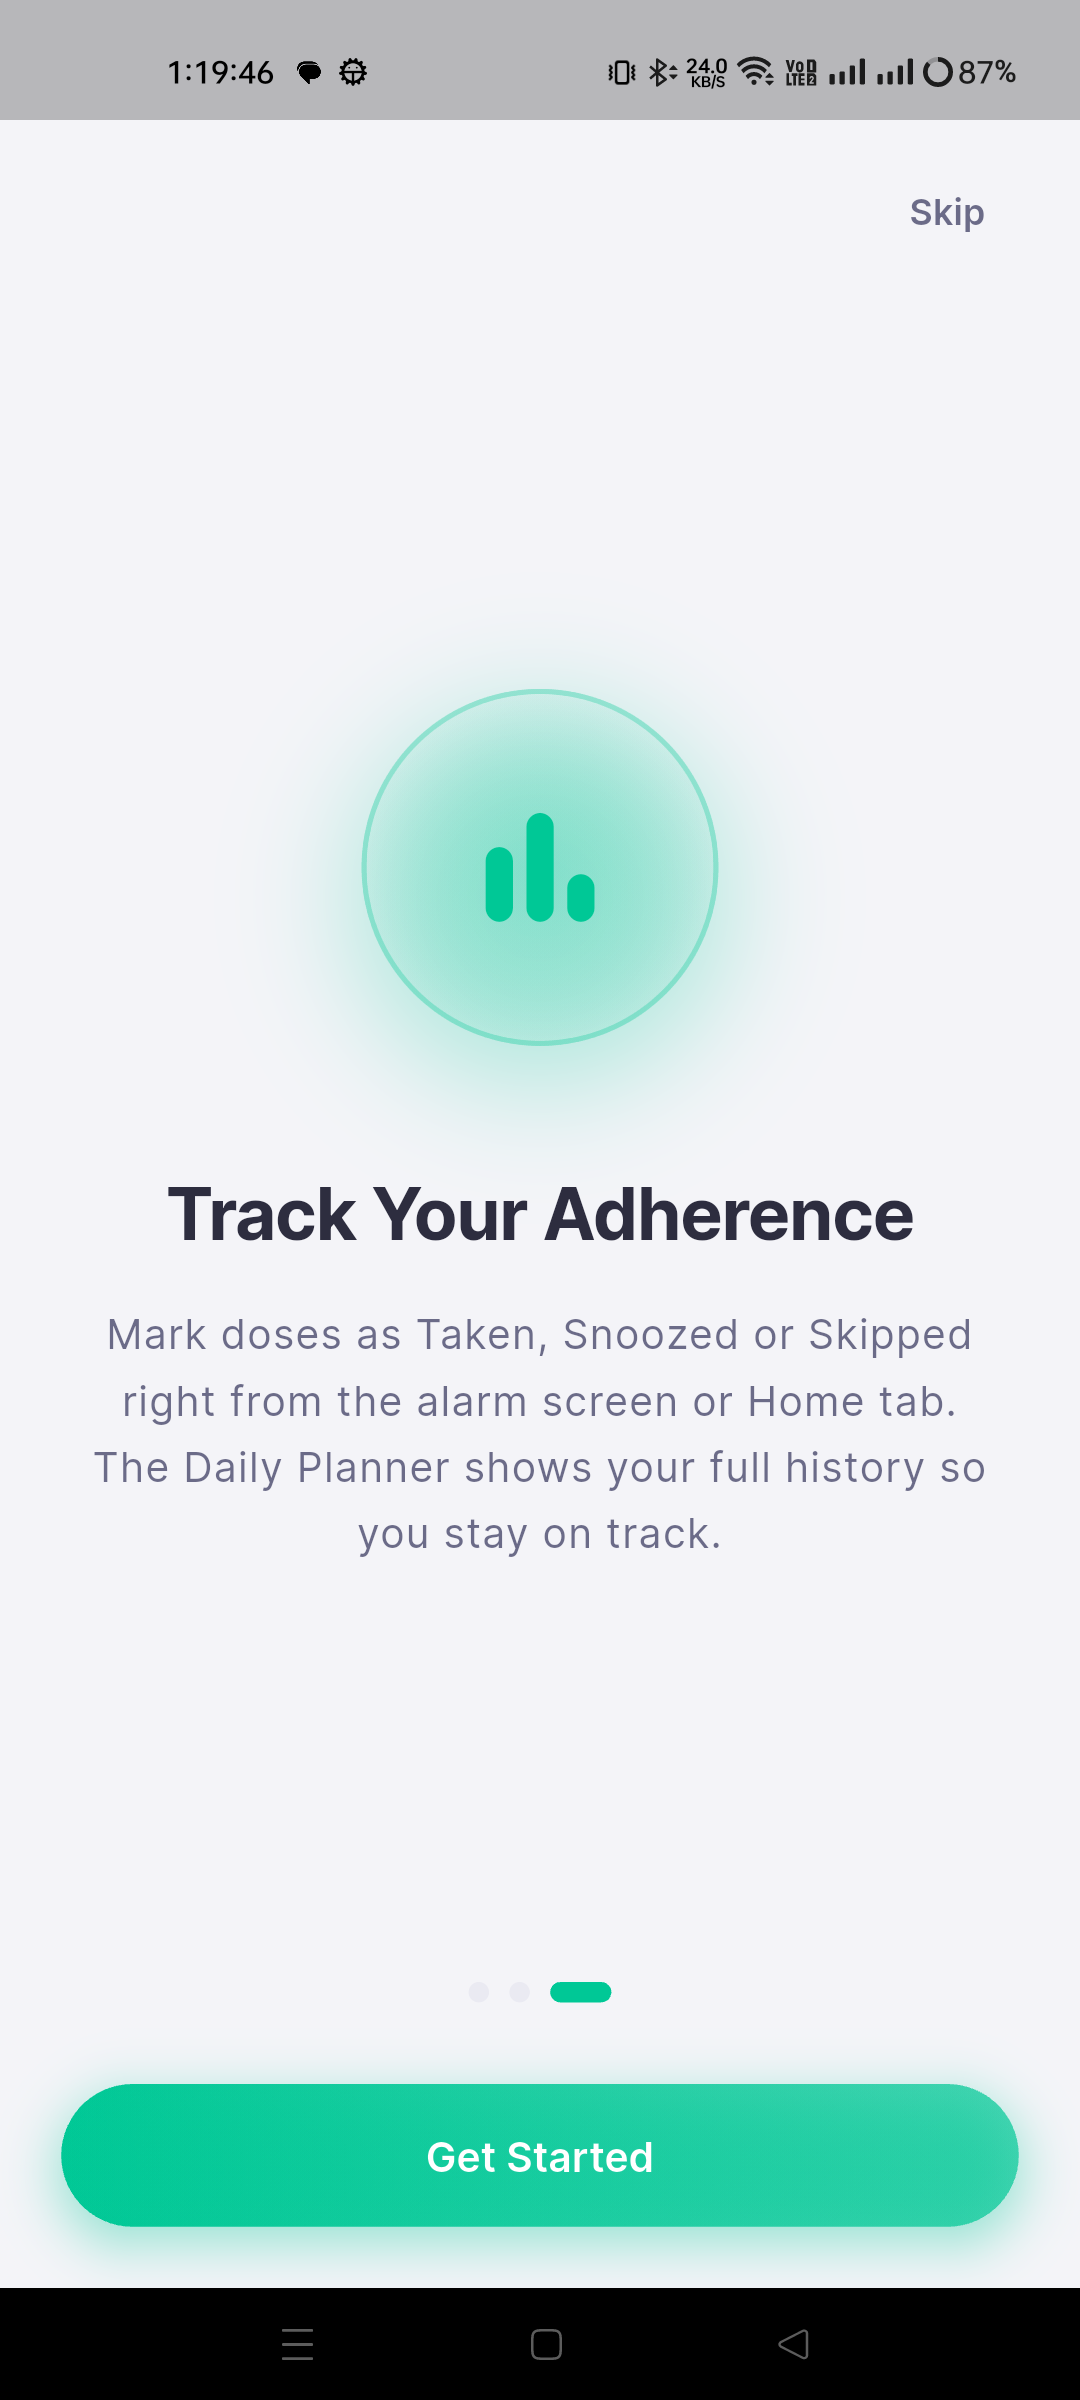
\includegraphics[width=0.32\textwidth]{screenshots/06_onboarding_3.png}
    \caption{Onboarding: Never Miss a Dose, Your Medicine Cabinet, Track Your Adherence}
\end{figure}

Right after, MedRemind asks for the permissions it needs to actually ring
alarms reliably: notifications, exact alarms, and an exemption from battery
optimization (so the OS doesn't kill the alarm in the background).

\begin{figure}[H]
    \centering
    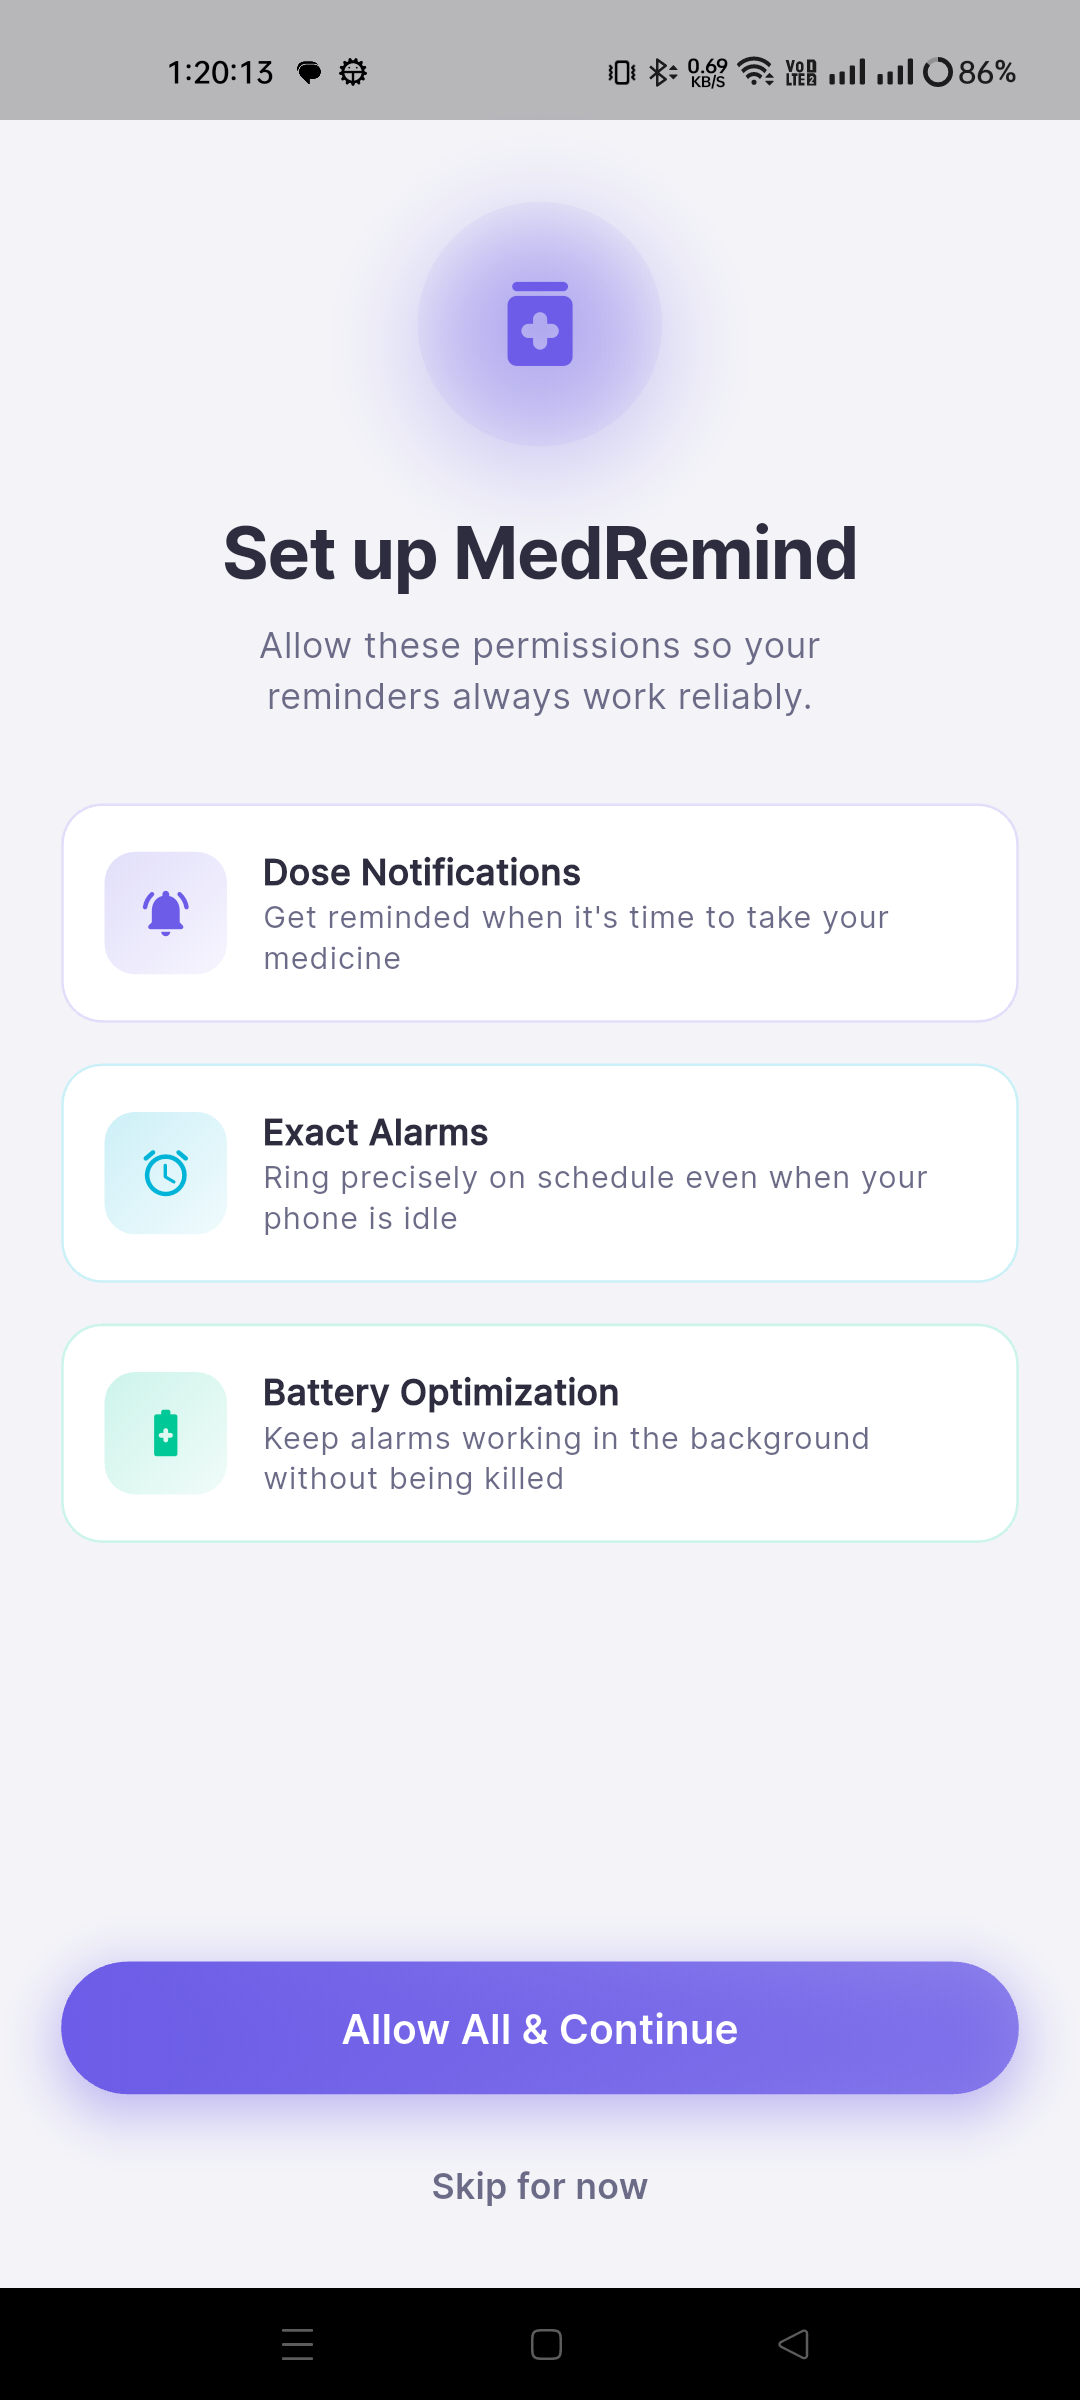
\includegraphics[width=0.45\textwidth]{screenshots/07_permissions.png}
    \caption{Set up MedRemind — permission requests}
\end{figure}

You can tap \textbf{Allow All \& Continue} to grant everything at once, or
\textbf{Skip for now} and grant permissions later from Settings. Skipping
these, especially \emph{Exact Alarms} and \emph{Battery Optimization}, may
cause reminders to ring late or not at all.

% ─────────────────────────────────────────────────────────────
\section{Home Screen}

The Home tab is what you land on after signing in. It shows:

\begin{itemize}[leftmargin=1.5em]
    \item A \textbf{Today's Pills} summary card with a progress ring.
    \item Filter chips: \emph{All / Morning / Afternoon / Evening / Night}.
    \item A 7-day date strip to jump to a different day.
    \item The list of doses due that day, each with \textbf{Taken},
        \textbf{Snooze}, and \textbf{Skip} actions.
\end{itemize}

Before any medicines are added, the Home screen shows an empty state
prompting you to add your first medicine.

\begin{figure}[H]
    \centering
    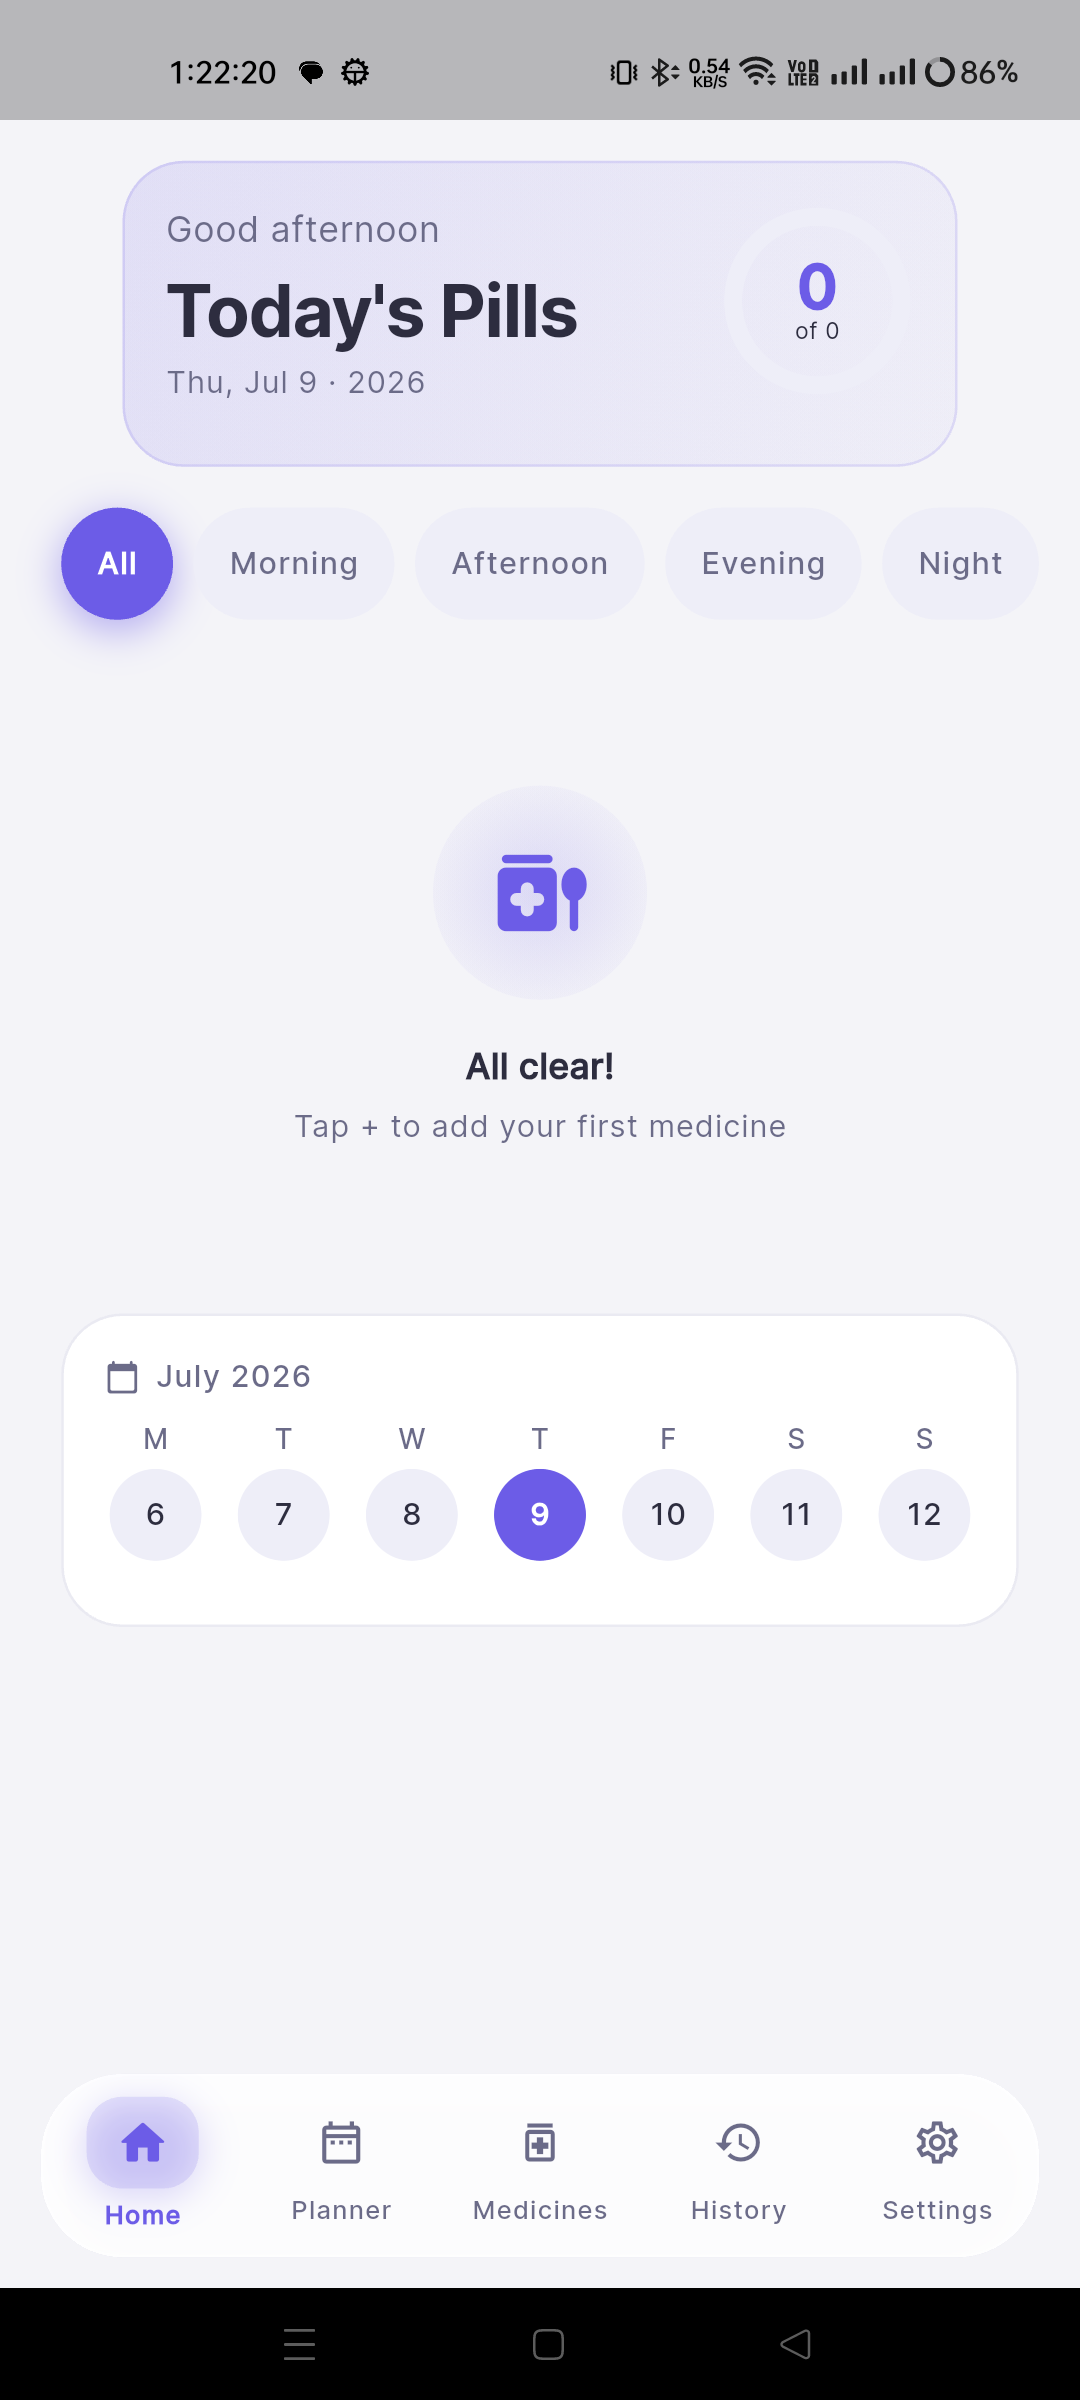
\includegraphics[width=0.45\textwidth]{screenshots/08_home_empty.png}
    \caption{Home tab — empty state}
\end{figure}

Once a dose group exists, its doses appear as cards on Home. Each dose card
lets you mark it Taken, Snooze it for a few minutes, or Skip it outright.

\begin{figure}[H]
    \centering
    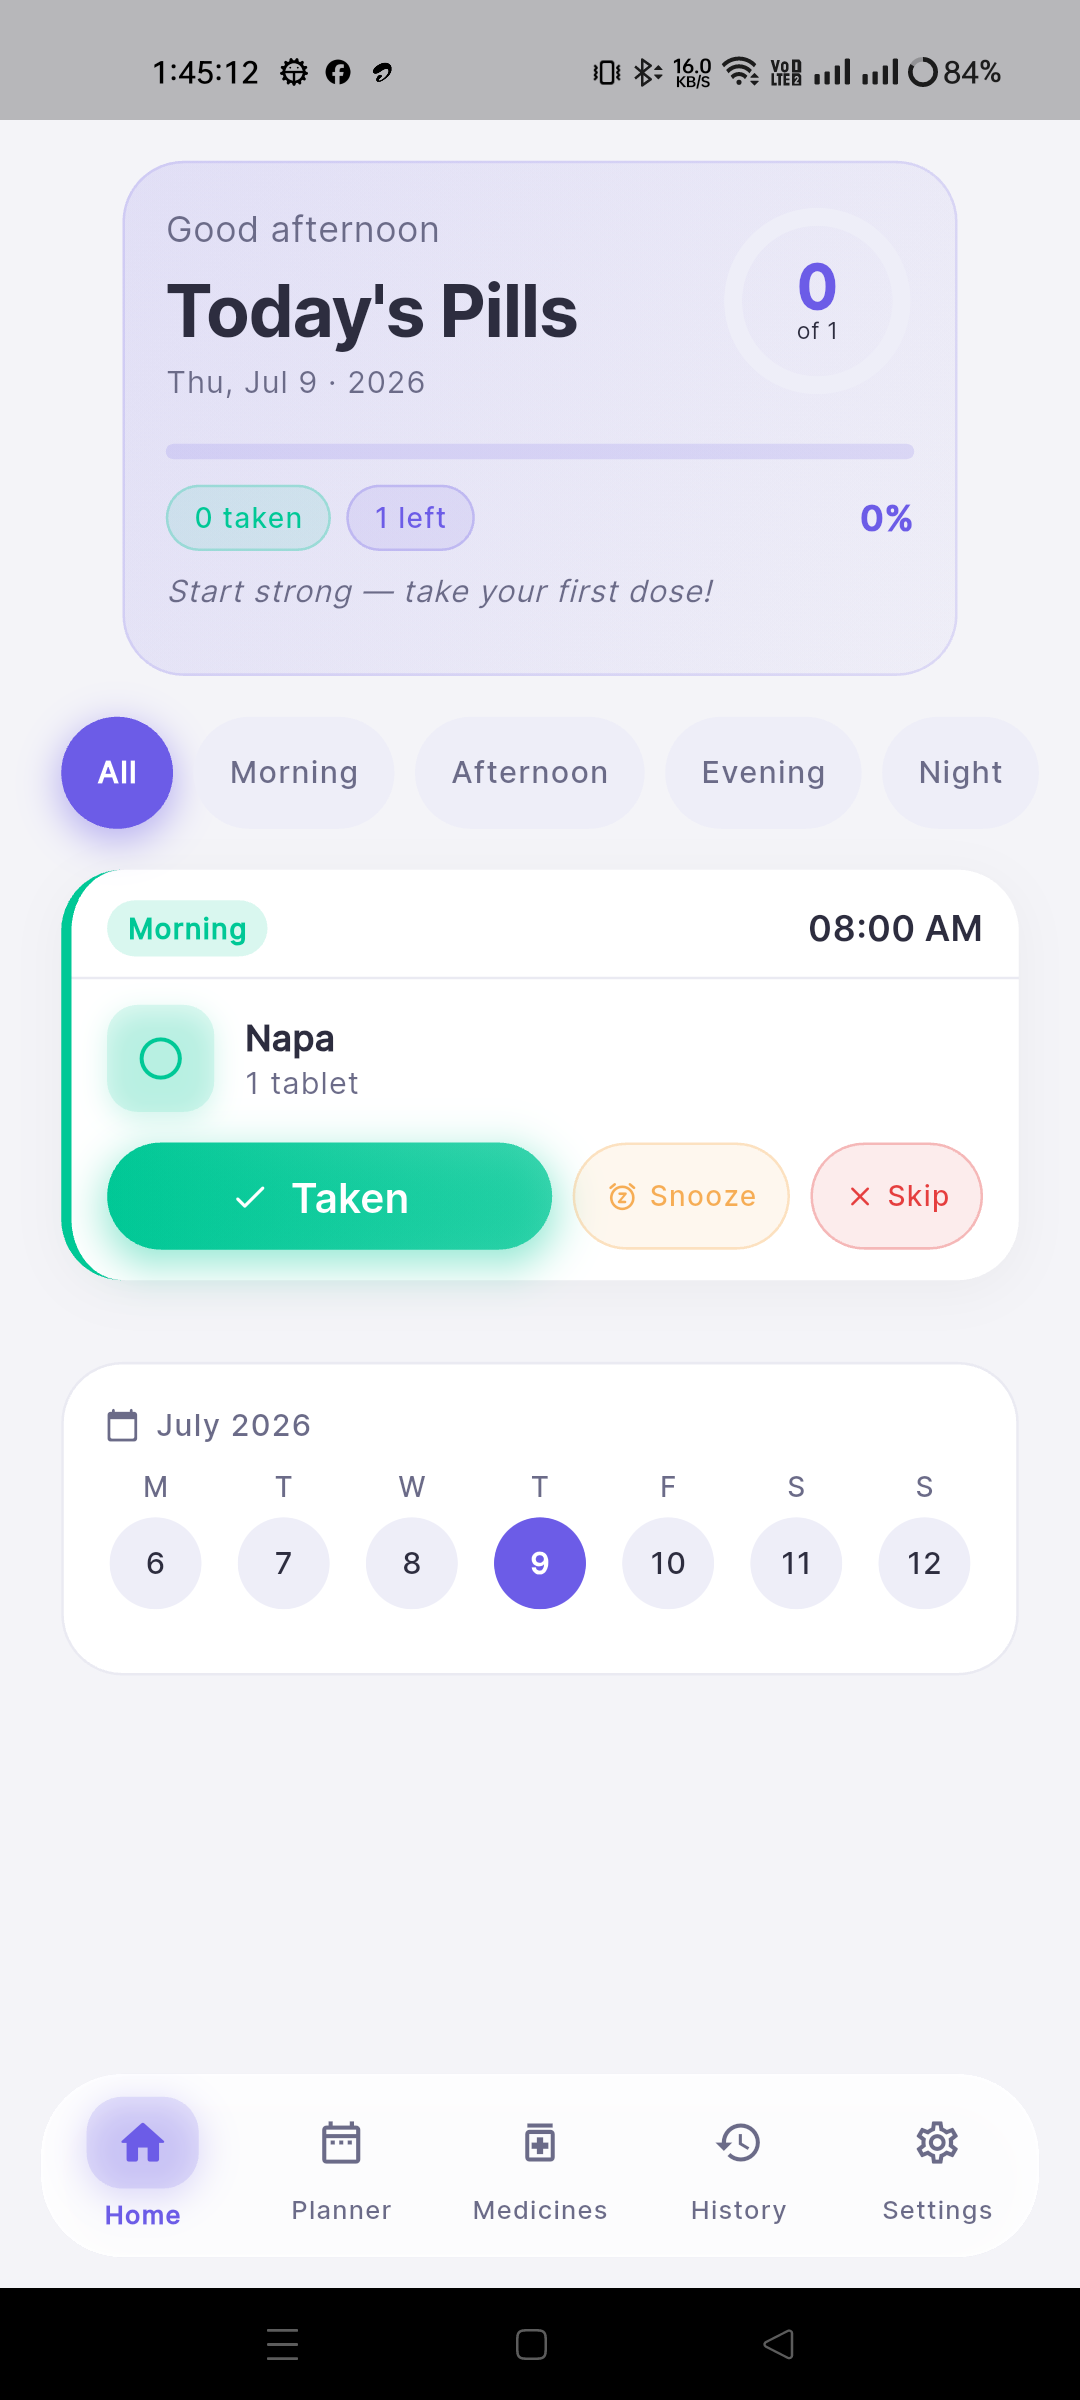
\includegraphics[width=0.45\textwidth]{screenshots/16_home_dose_card.png}
    \caption{A due dose, with Taken / Snooze / Skip actions}
\end{figure}

Once every dose for the day is marked Taken, the progress ring fills to
100\% and the day's remaining schedule (today's completed doses, and
tomorrow's upcoming ones) is shown below.

\begin{figure}[H]
    \centering
    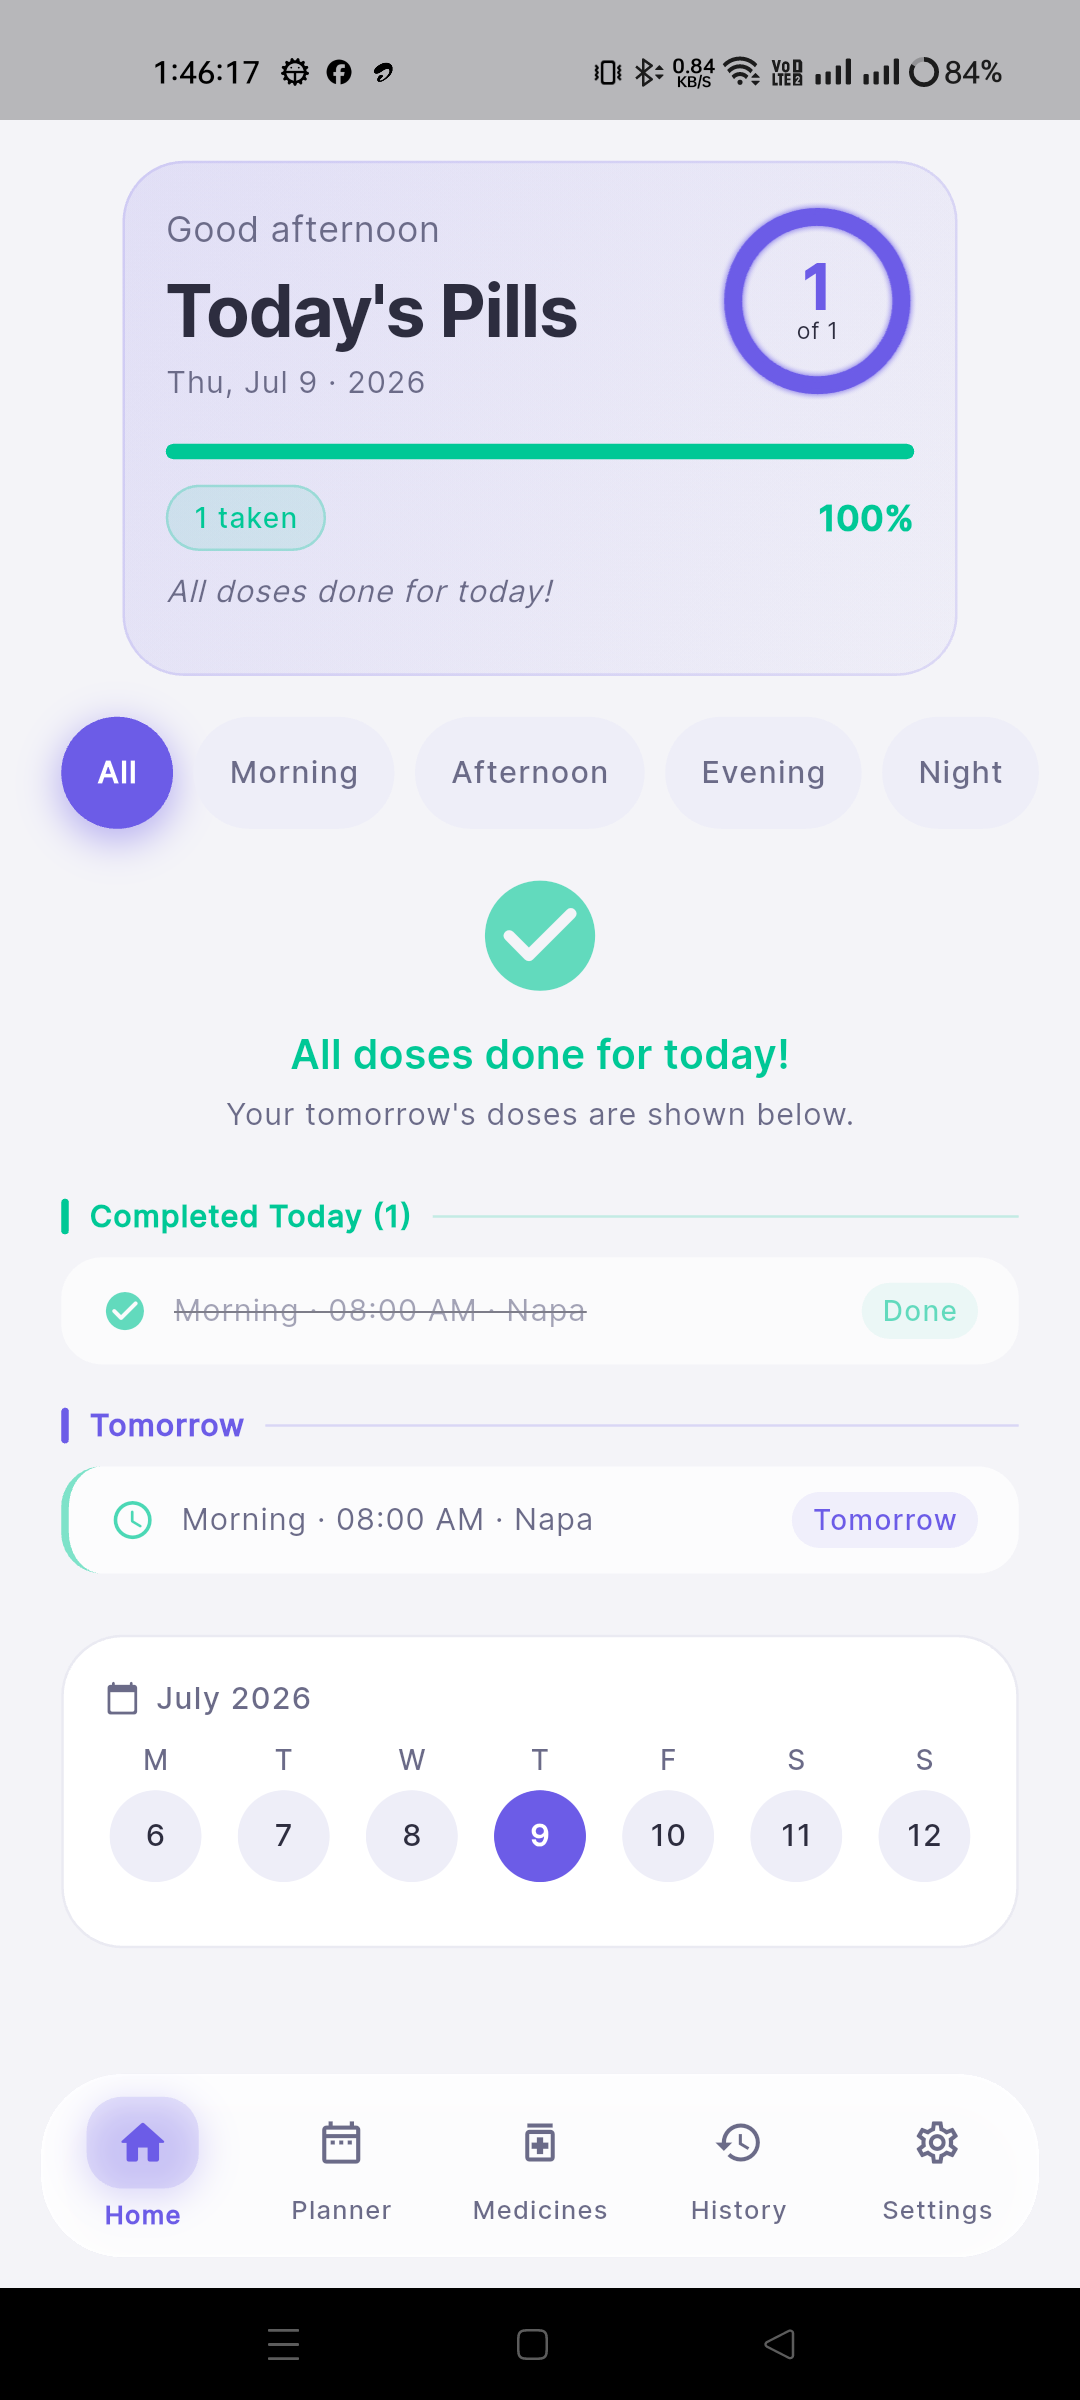
\includegraphics[width=0.45\textwidth]{screenshots/17_home_completed.png}
    \caption{All doses done for today}
\end{figure}

% ─────────────────────────────────────────────────────────────
\section{Medicine Cabinet}

The \textbf{Medicines} tab is where you manage what you take and when. It
has two sub-tabs: \emph{Medicines} (the raw list of medicines you take) and
\emph{Schedules} (the dose groups that actually trigger alarms).

\subsection{Adding a Medicine}

Tap \textbf{+ Add Medicine} from the empty Medicines list to open the add
form.

\begin{figure}[H]
    \centering
    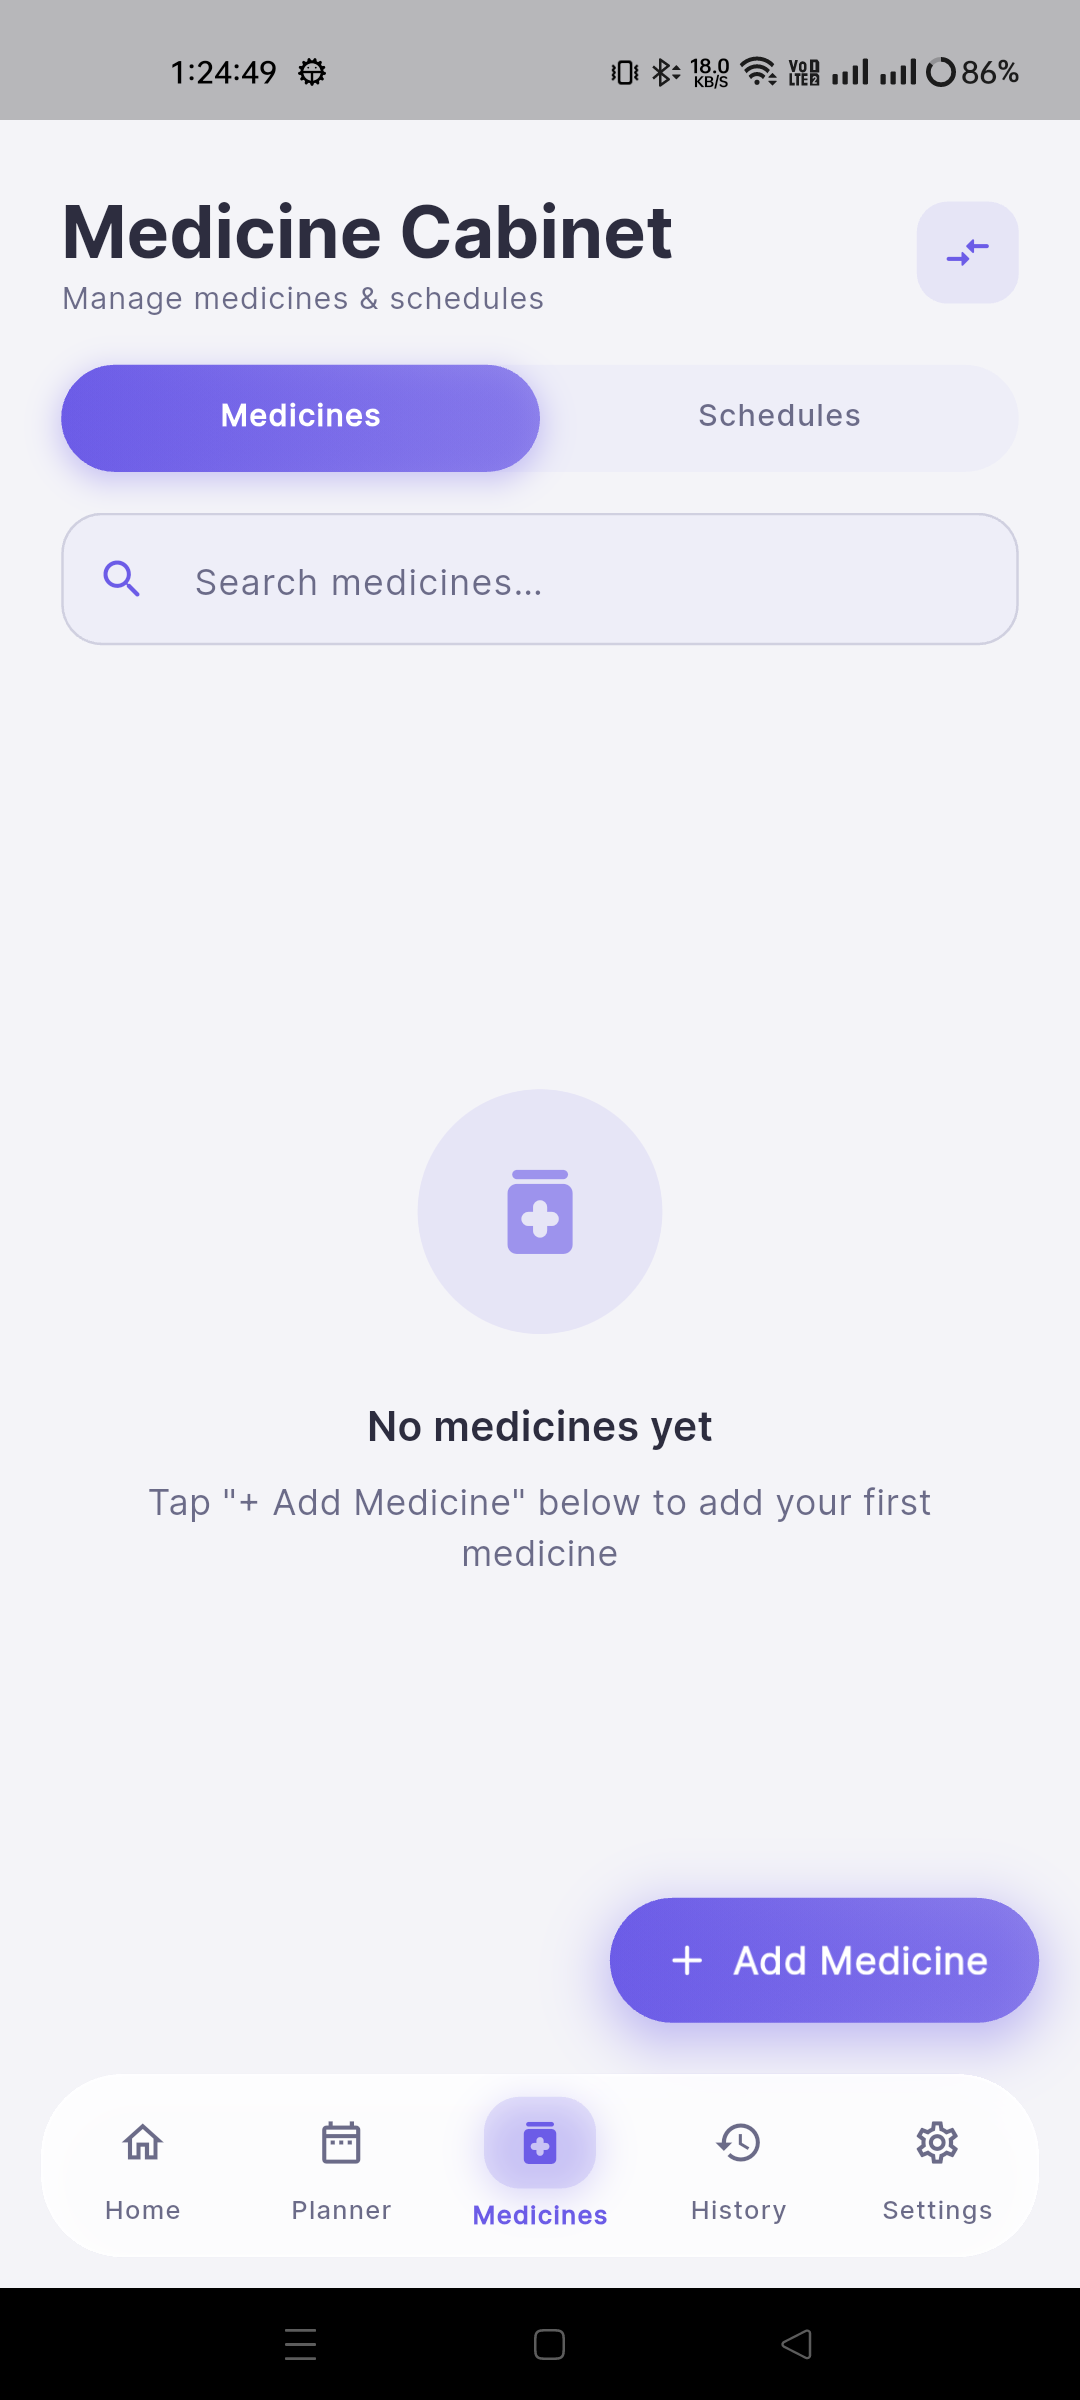
\includegraphics[width=0.45\textwidth]{screenshots/09_medicine_cabinet_empty.png}\hfill
    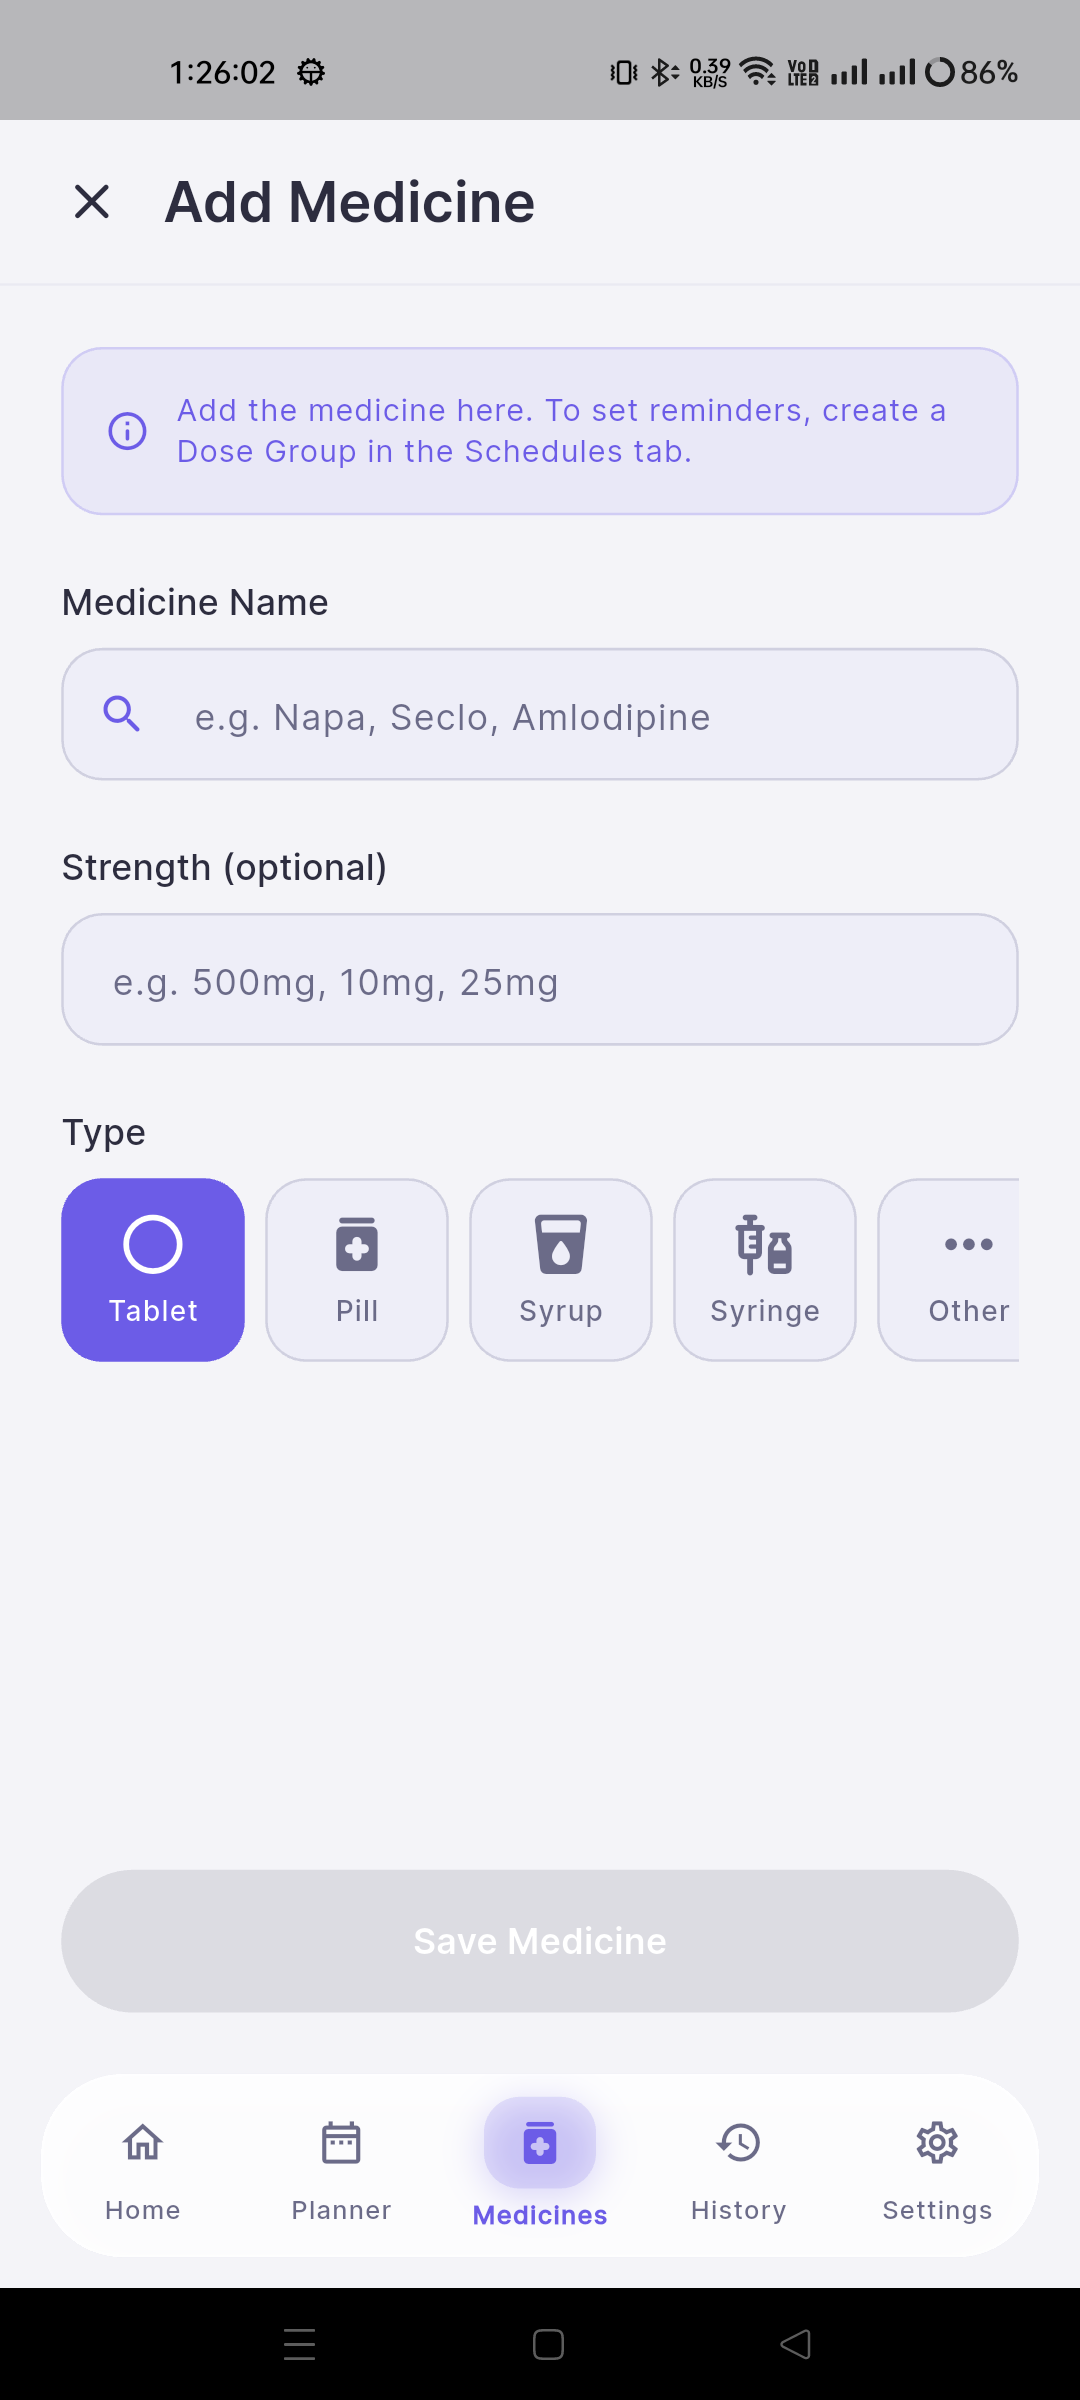
\includegraphics[width=0.45\textwidth]{screenshots/10_add_medicine.png}
    \caption{Medicine Cabinet (empty) and the Add Medicine form}
\end{figure}

As you type a medicine name, MedRemind suggests matches from a built-in
database of common Bangladeshi brand names, along with the generic drug name
(e.g. \emph{Napa} $\rightarrow$ Generic: Paracetamol). You can optionally set
a strength (e.g. 500mg) and a form (Tablet, Pill, Syrup, Syringe, or Other).

\begin{figure}[H]
    \centering
    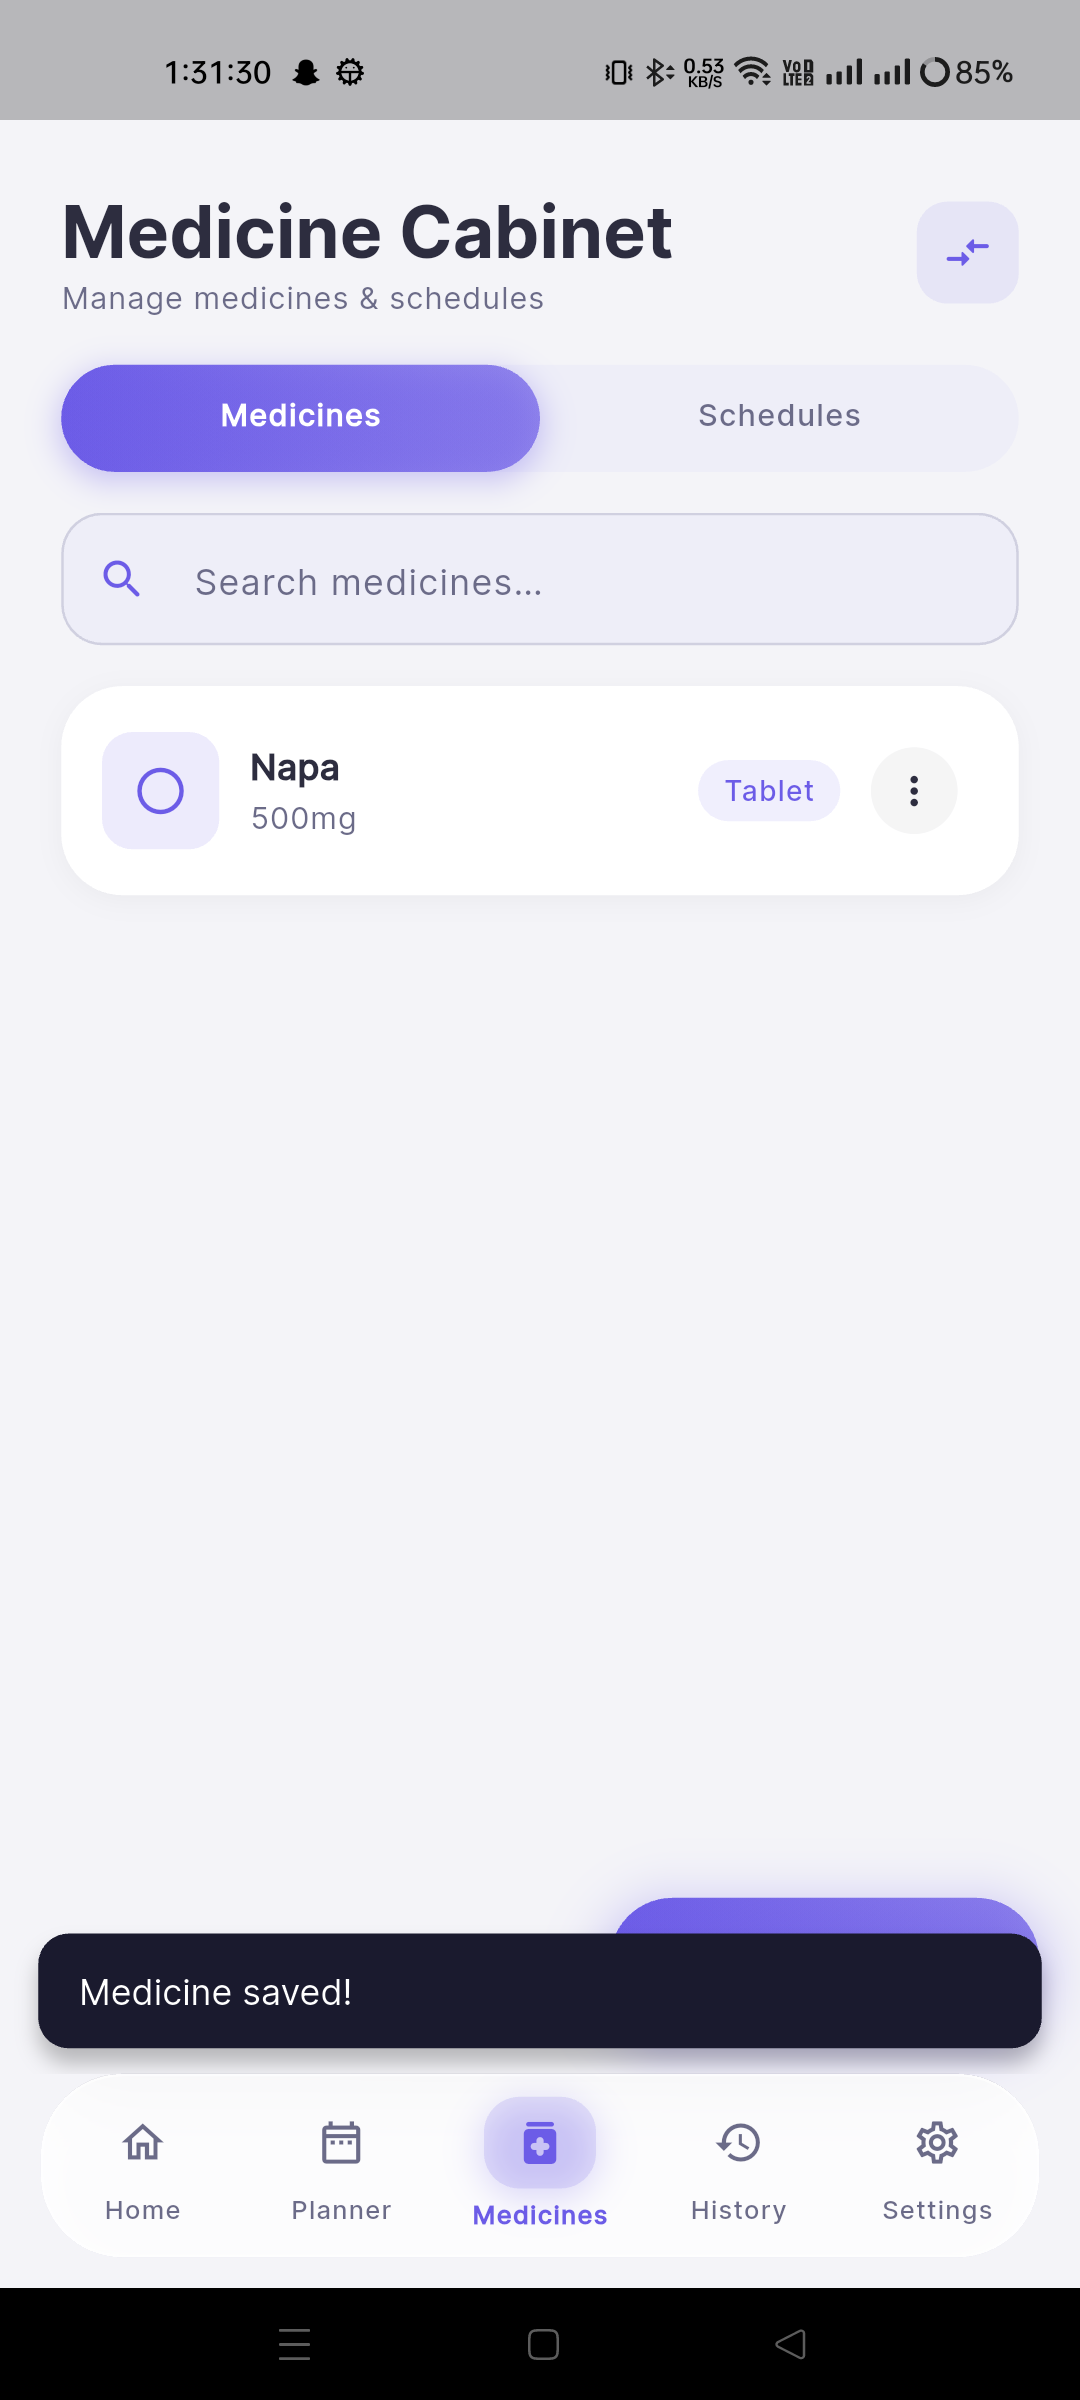
\includegraphics[width=0.45\textwidth]{screenshots/11_medicine_added.png}
    \caption{Medicine saved and listed in the cabinet}
\end{figure}

\textbf{Note:} adding a medicine here does \emph{not} by itself create any
reminders. To actually get an alarm, you need to add the medicine to a
\emph{Dose Group}, covered next.

\subsection{Creating a Dose Group}

Switch to the \textbf{Schedules} sub-tab and tap \textbf{+ New Group}. A dose
group bundles together:

\begin{itemize}[leftmargin=1.5em]
    \item A \textbf{Dose Time} label (Morning / Afternoon / Evening / Night)
        — purely descriptive, shown throughout the app.
    \item An exact \textbf{Alarm Time}.
    \item An optional \textbf{Meal Relation} (No preference / Before meal /
        After meal) — shown as a note on the reminder.
    \item \textbf{Repeat Days} — every day by default, or specific weekdays.
    \item One or more \textbf{Medicines}, each with its own quantity.
\end{itemize}

\begin{figure}[H]
    \centering
    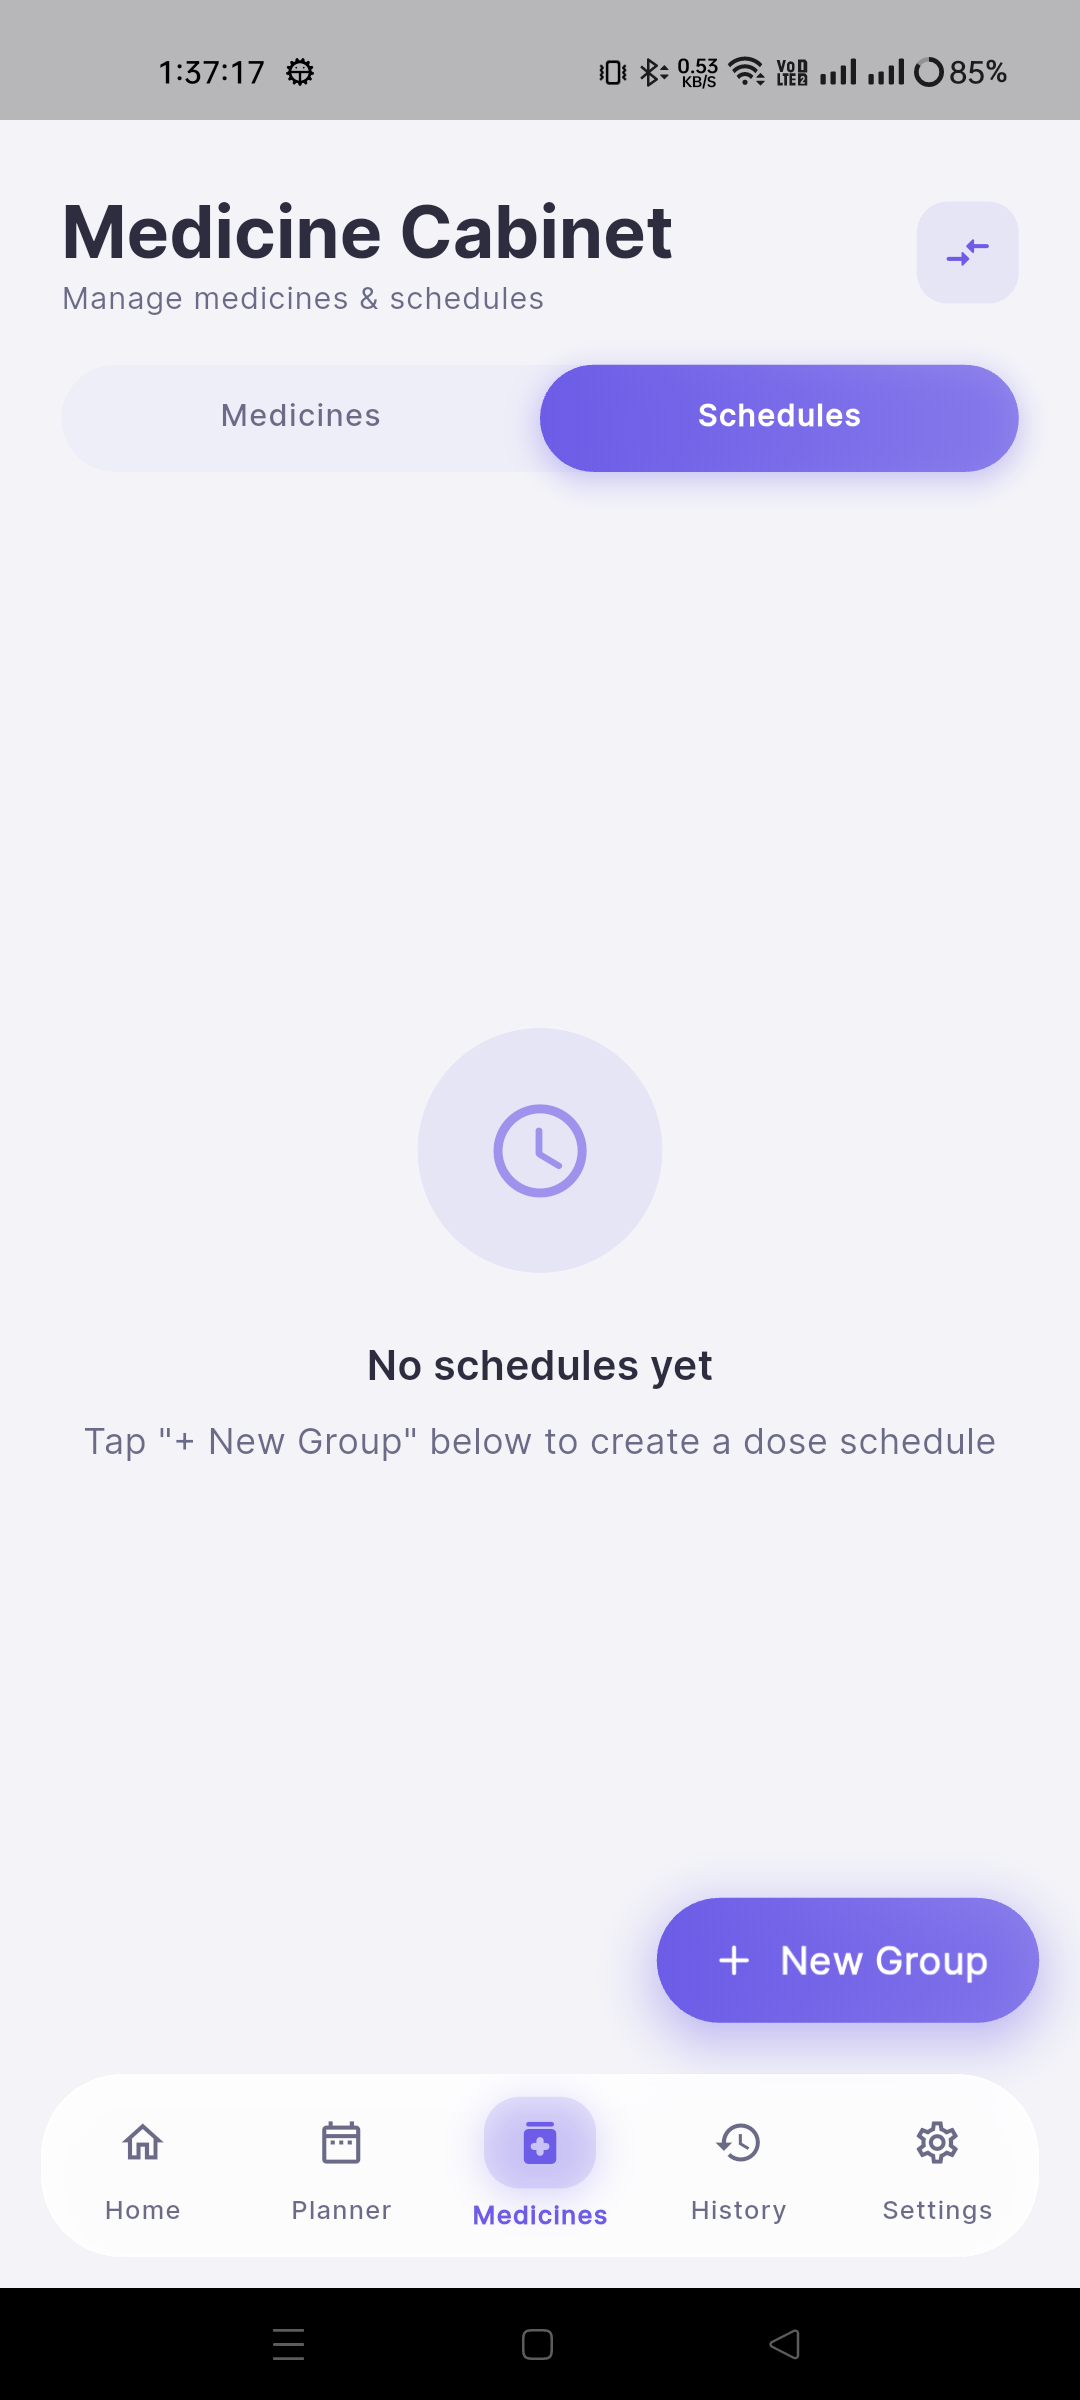
\includegraphics[width=0.45\textwidth]{screenshots/12_schedules_empty.png}\hfill
    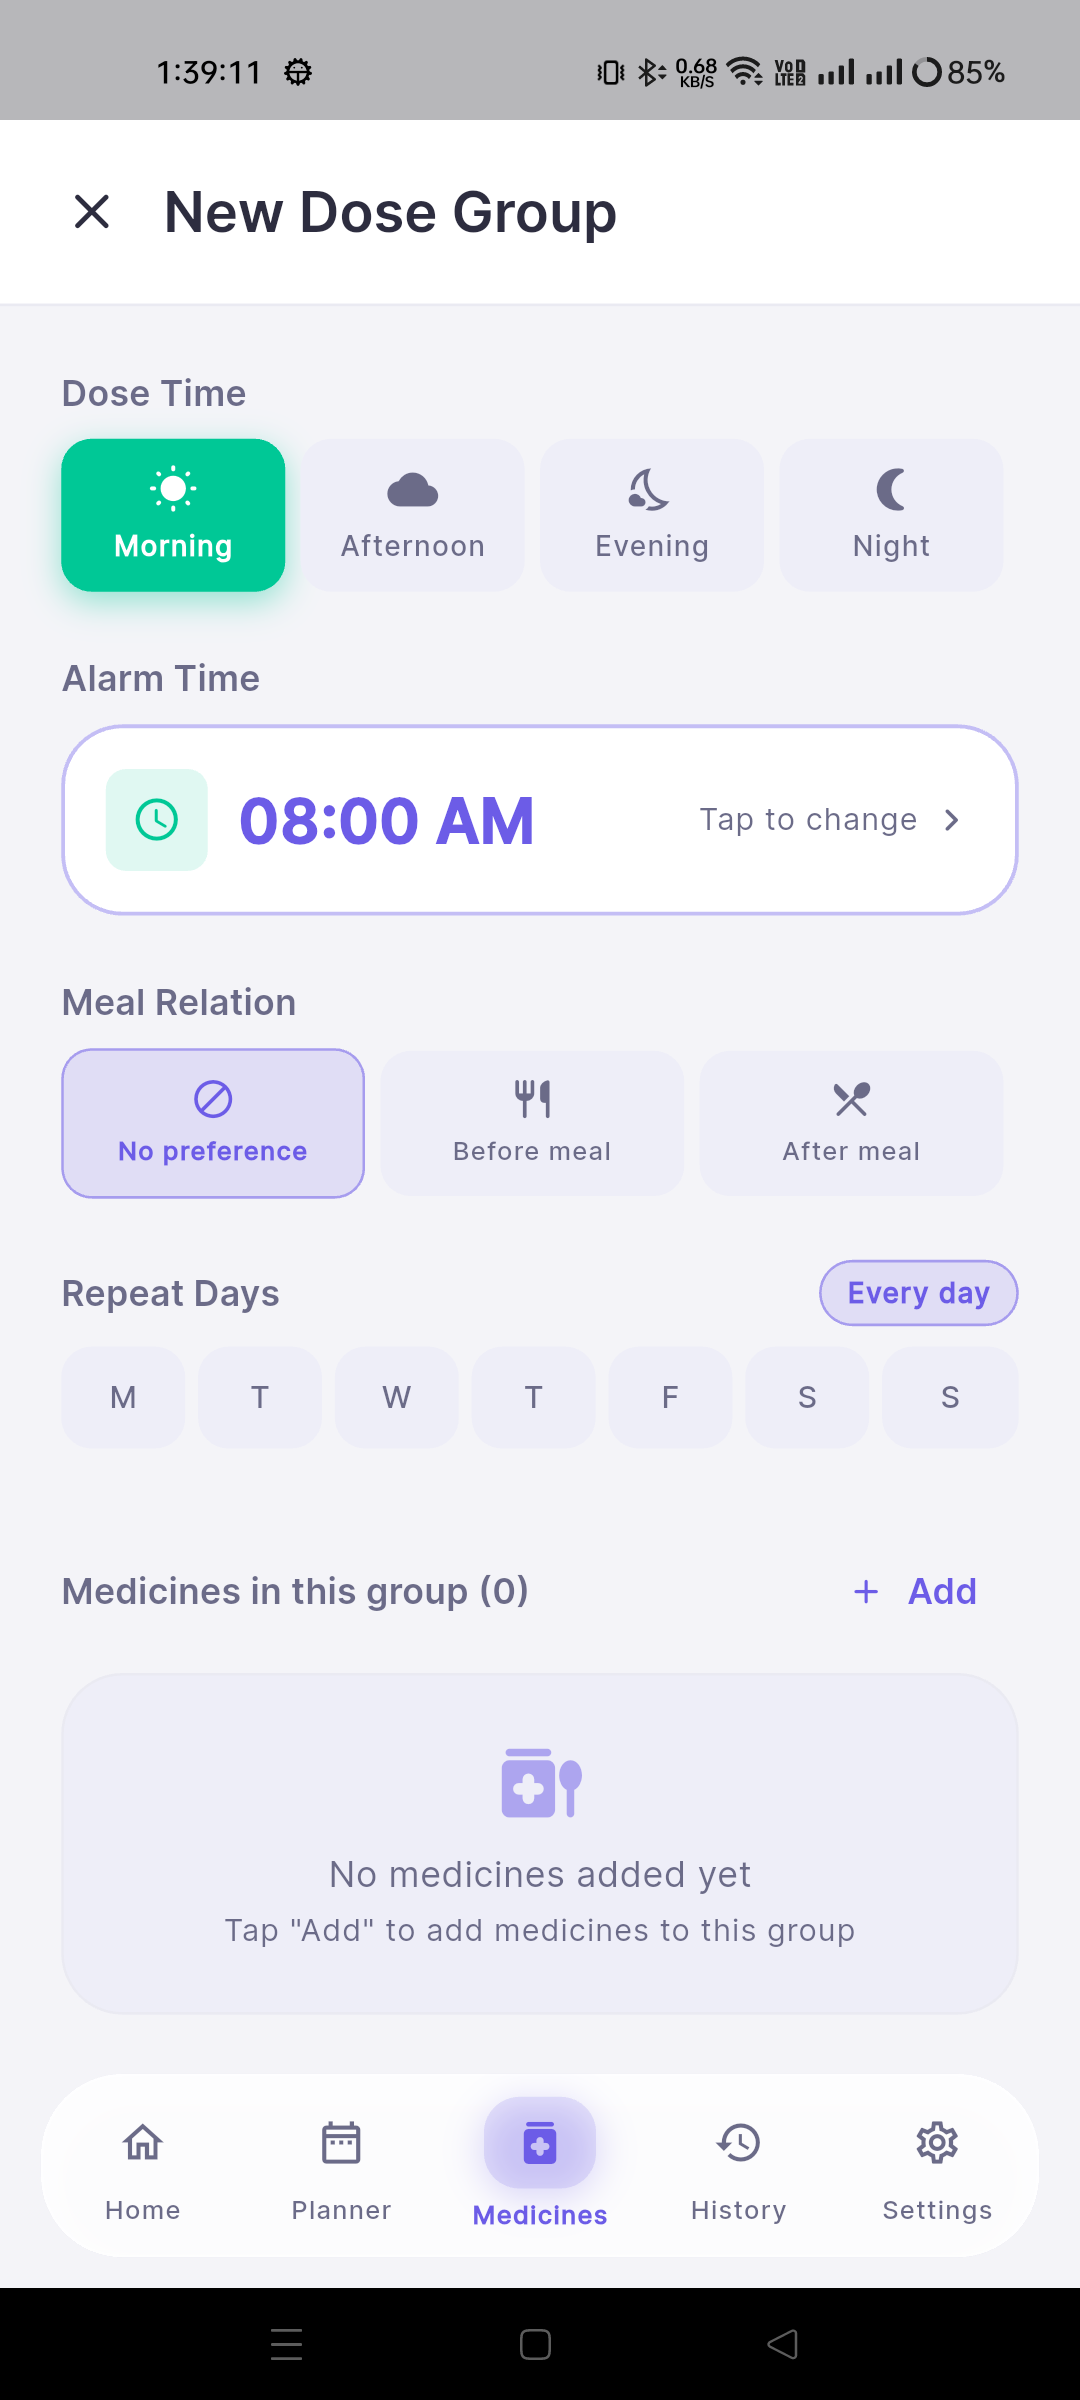
\includegraphics[width=0.45\textwidth]{screenshots/13_new_dose_group.png}
    \caption{Schedules tab (empty) and the New Dose Group form}
\end{figure}

Tap \textbf{Add} under "Medicines in this group" to pick from your cabinet.
Each added medicine gets its own $-$/$+$ quantity stepper.

\begin{figure}[H]
    \centering
    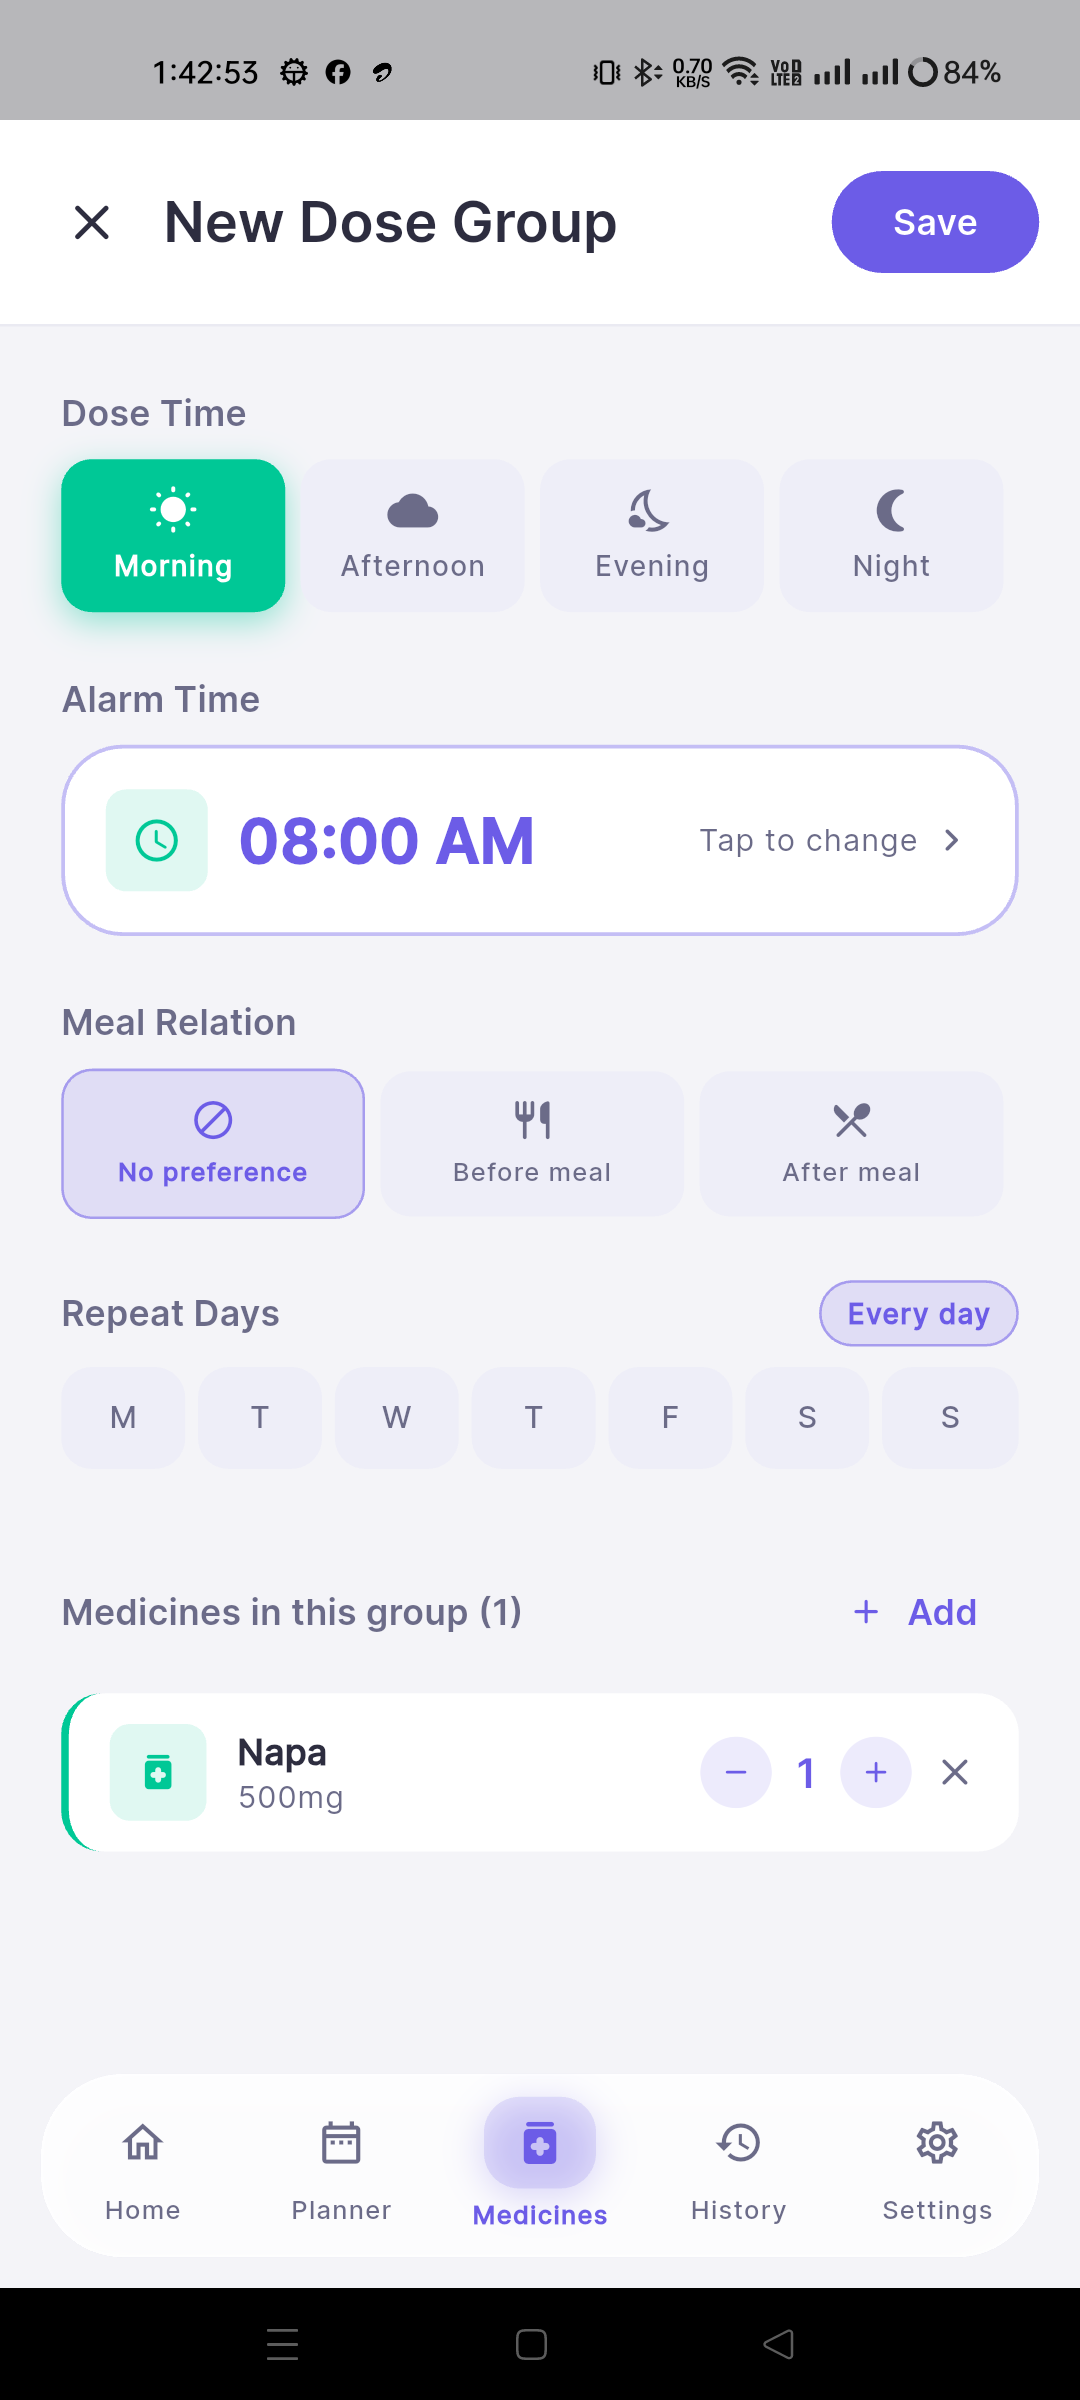
\includegraphics[width=0.45\textwidth]{screenshots/14_dose_group_medicine_added.png}
    \caption{A medicine added to the dose group, with quantity control}
\end{figure}

Once saved, the group appears in the Schedules list, and its dose will now
show up on the Home tab and in the Daily Planner at the time you chose.

\begin{figure}[H]
    \centering
    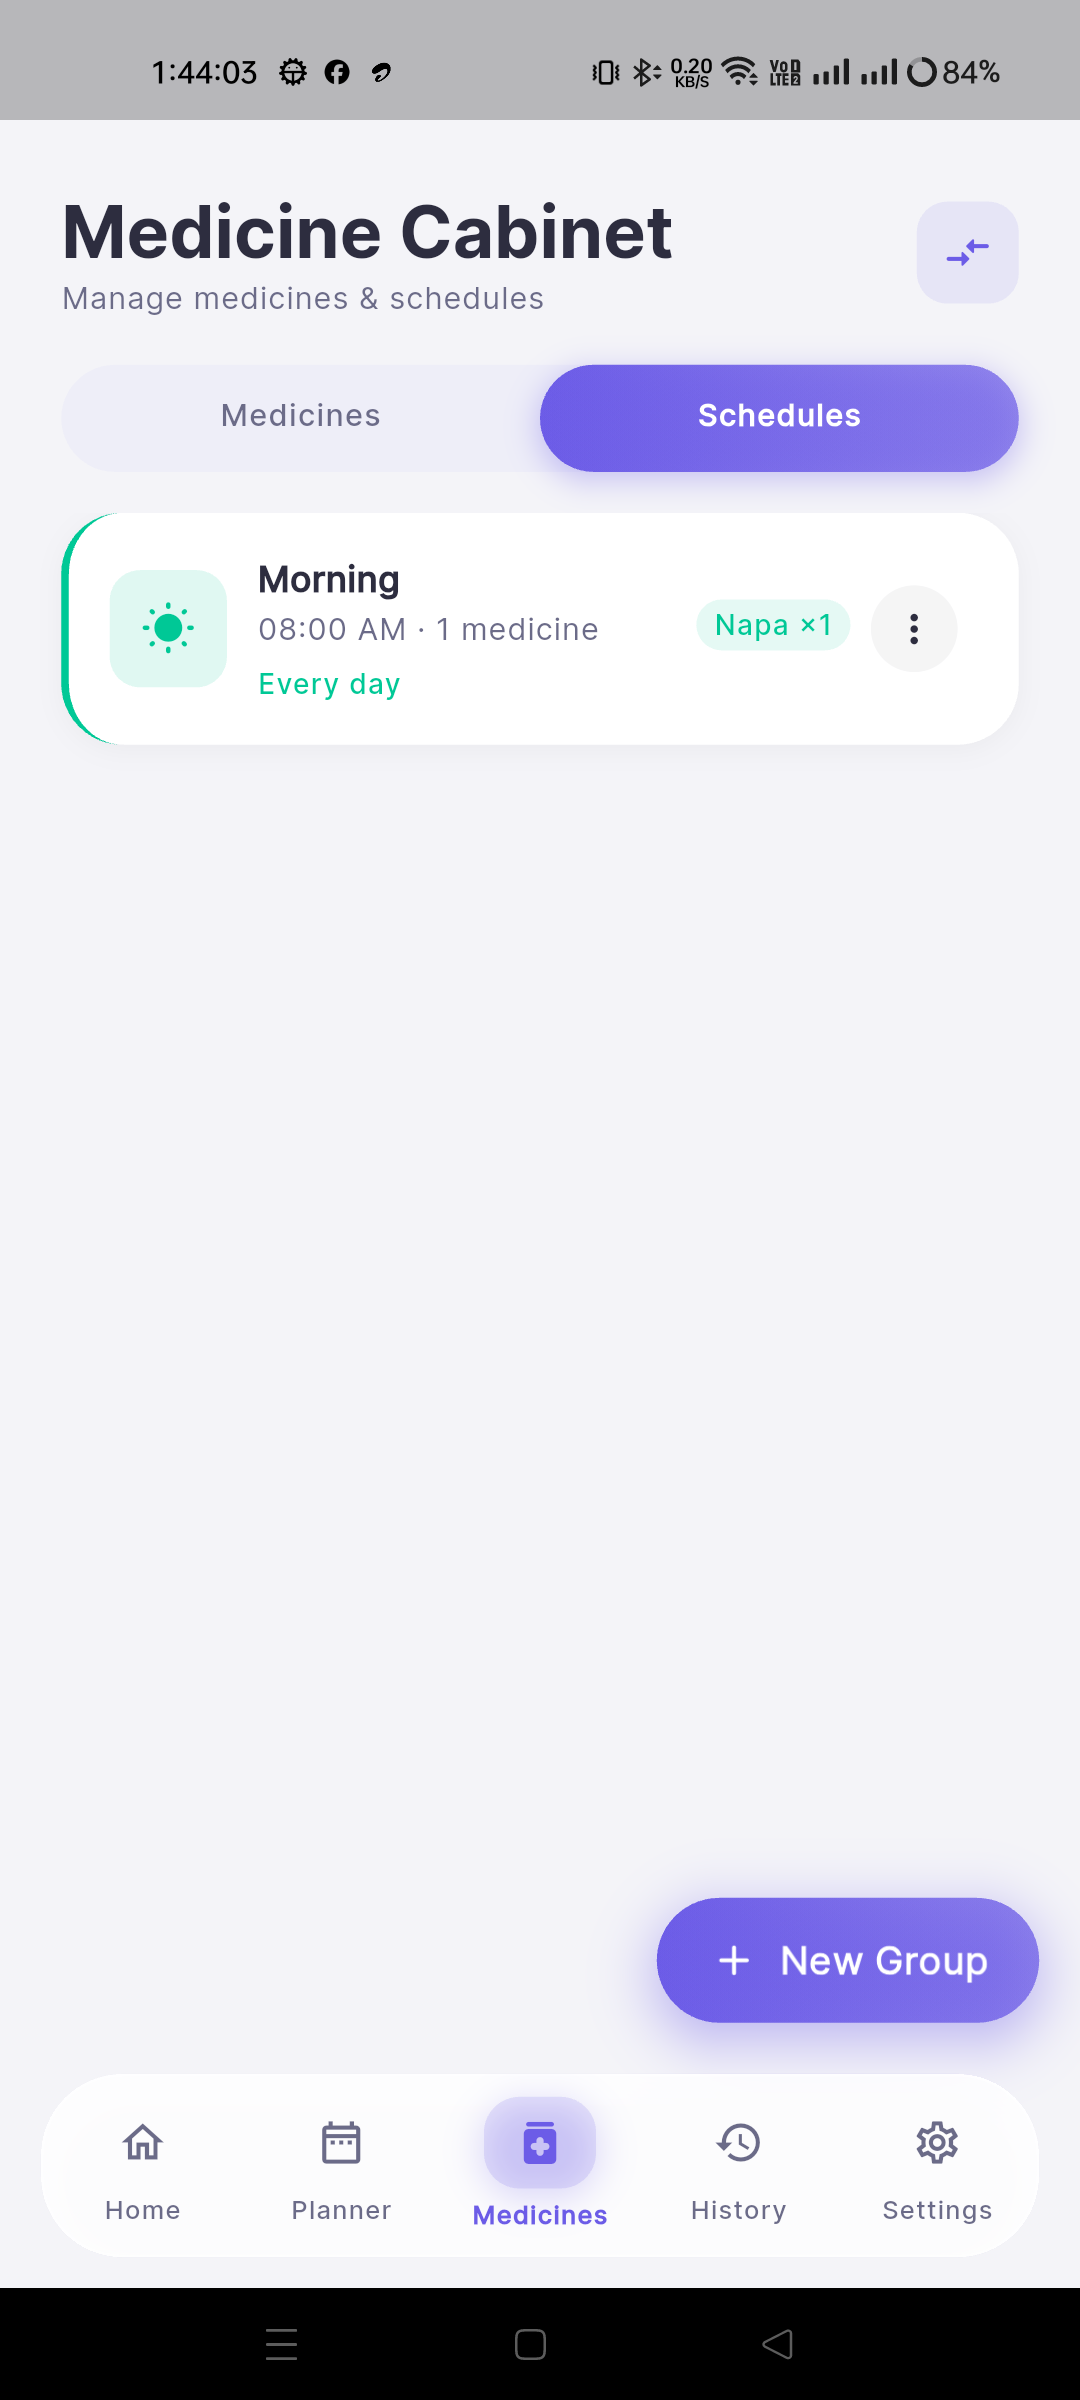
\includegraphics[width=0.45\textwidth]{screenshots/15_dose_group_saved.png}
    \caption{Saved dose group: Morning, 08:00\,AM, Napa \texttimes 1, every day}
\end{figure}

% ─────────────────────────────────────────────────────────────
\section{The Alarm}

When a dose group's alarm time arrives, MedRemind shows a full-screen alarm
— even over the lock screen or another app — with the medicine name and
quantity, and three actions: \textbf{Dismiss — Taken}, \textbf{Snooze 5 min},
and \textbf{Skip}. Swiping up also marks it Taken.

\begin{figure}[H]
    \centering
    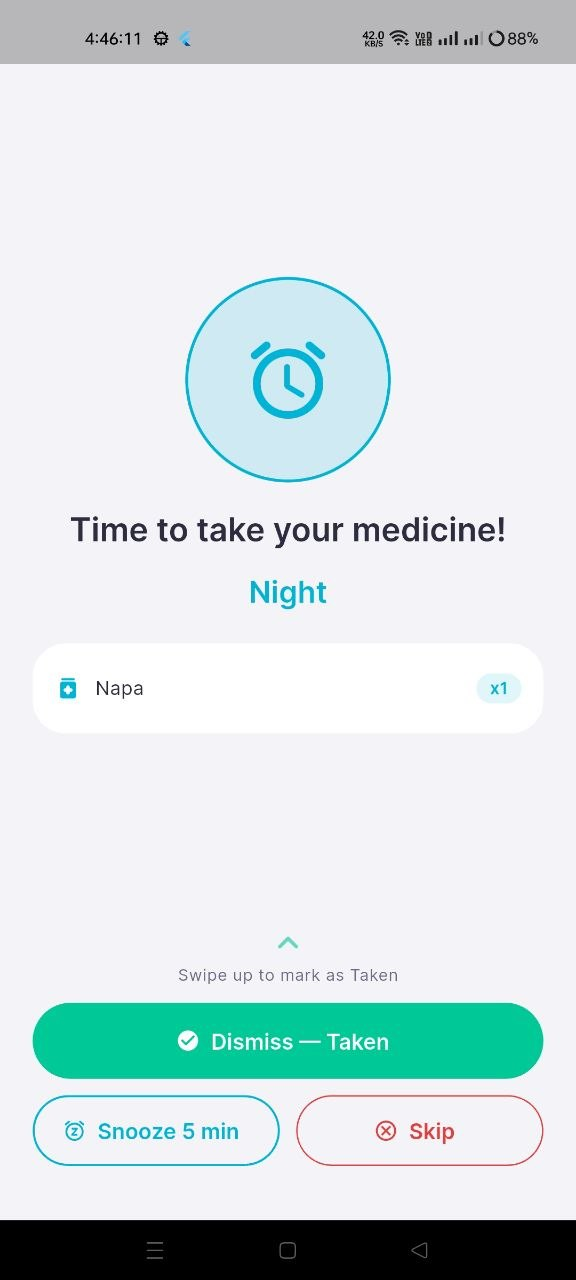
\includegraphics[width=0.4\textwidth]{screenshots/22_alarm_screen.png}
    \caption{Full-screen medicine alarm}
\end{figure}

If you don't see or act on the alarm right away, a regular notification is
also posted with the same three actions (Dismiss/Taken, Snooze, Skip)
available directly from the notification shade.

\begin{figure}[H]
    \centering
    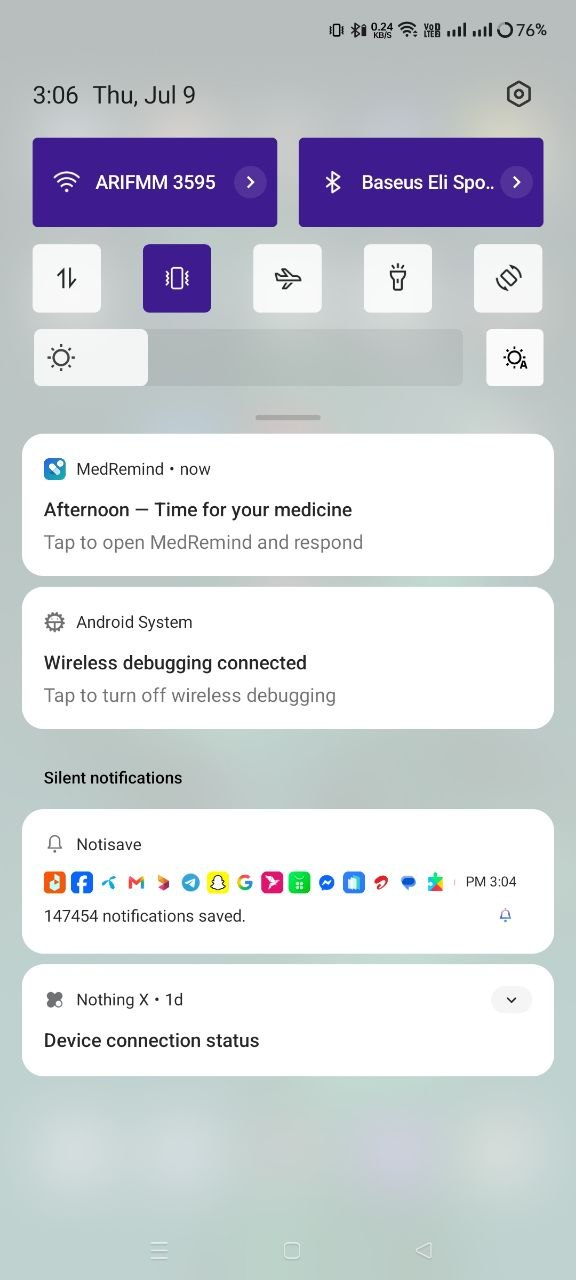
\includegraphics[width=0.4\textwidth]{screenshots/23_notification.jpg}
    \caption{Medicine alarm notification, actionable without opening the app}
\end{figure}

% ─────────────────────────────────────────────────────────────
\section{Daily Planner}

The \textbf{Planner} tab shows a full month calendar. Each day carries a
coloured dot summarizing that day's adherence:

\begin{itemize}[leftmargin=1.5em]
    \item \textcolor[HTML]{2ECC71}{\textbf{Green}} — All doses taken
    \item \textcolor[HTML]{F5A623}{\textbf{Orange}} — Partial (some doses taken, some not)
    \item \textcolor[HTML]{E74C3C}{\textbf{Red}} — Missed
    \item \textcolor[HTML]{9B8CF2}{\textbf{Purple}} — Scheduled (future day)
\end{itemize}

Selecting a day shows a summary card and the full list of that day's doses
with their status.

\begin{figure}[H]
    \centering
    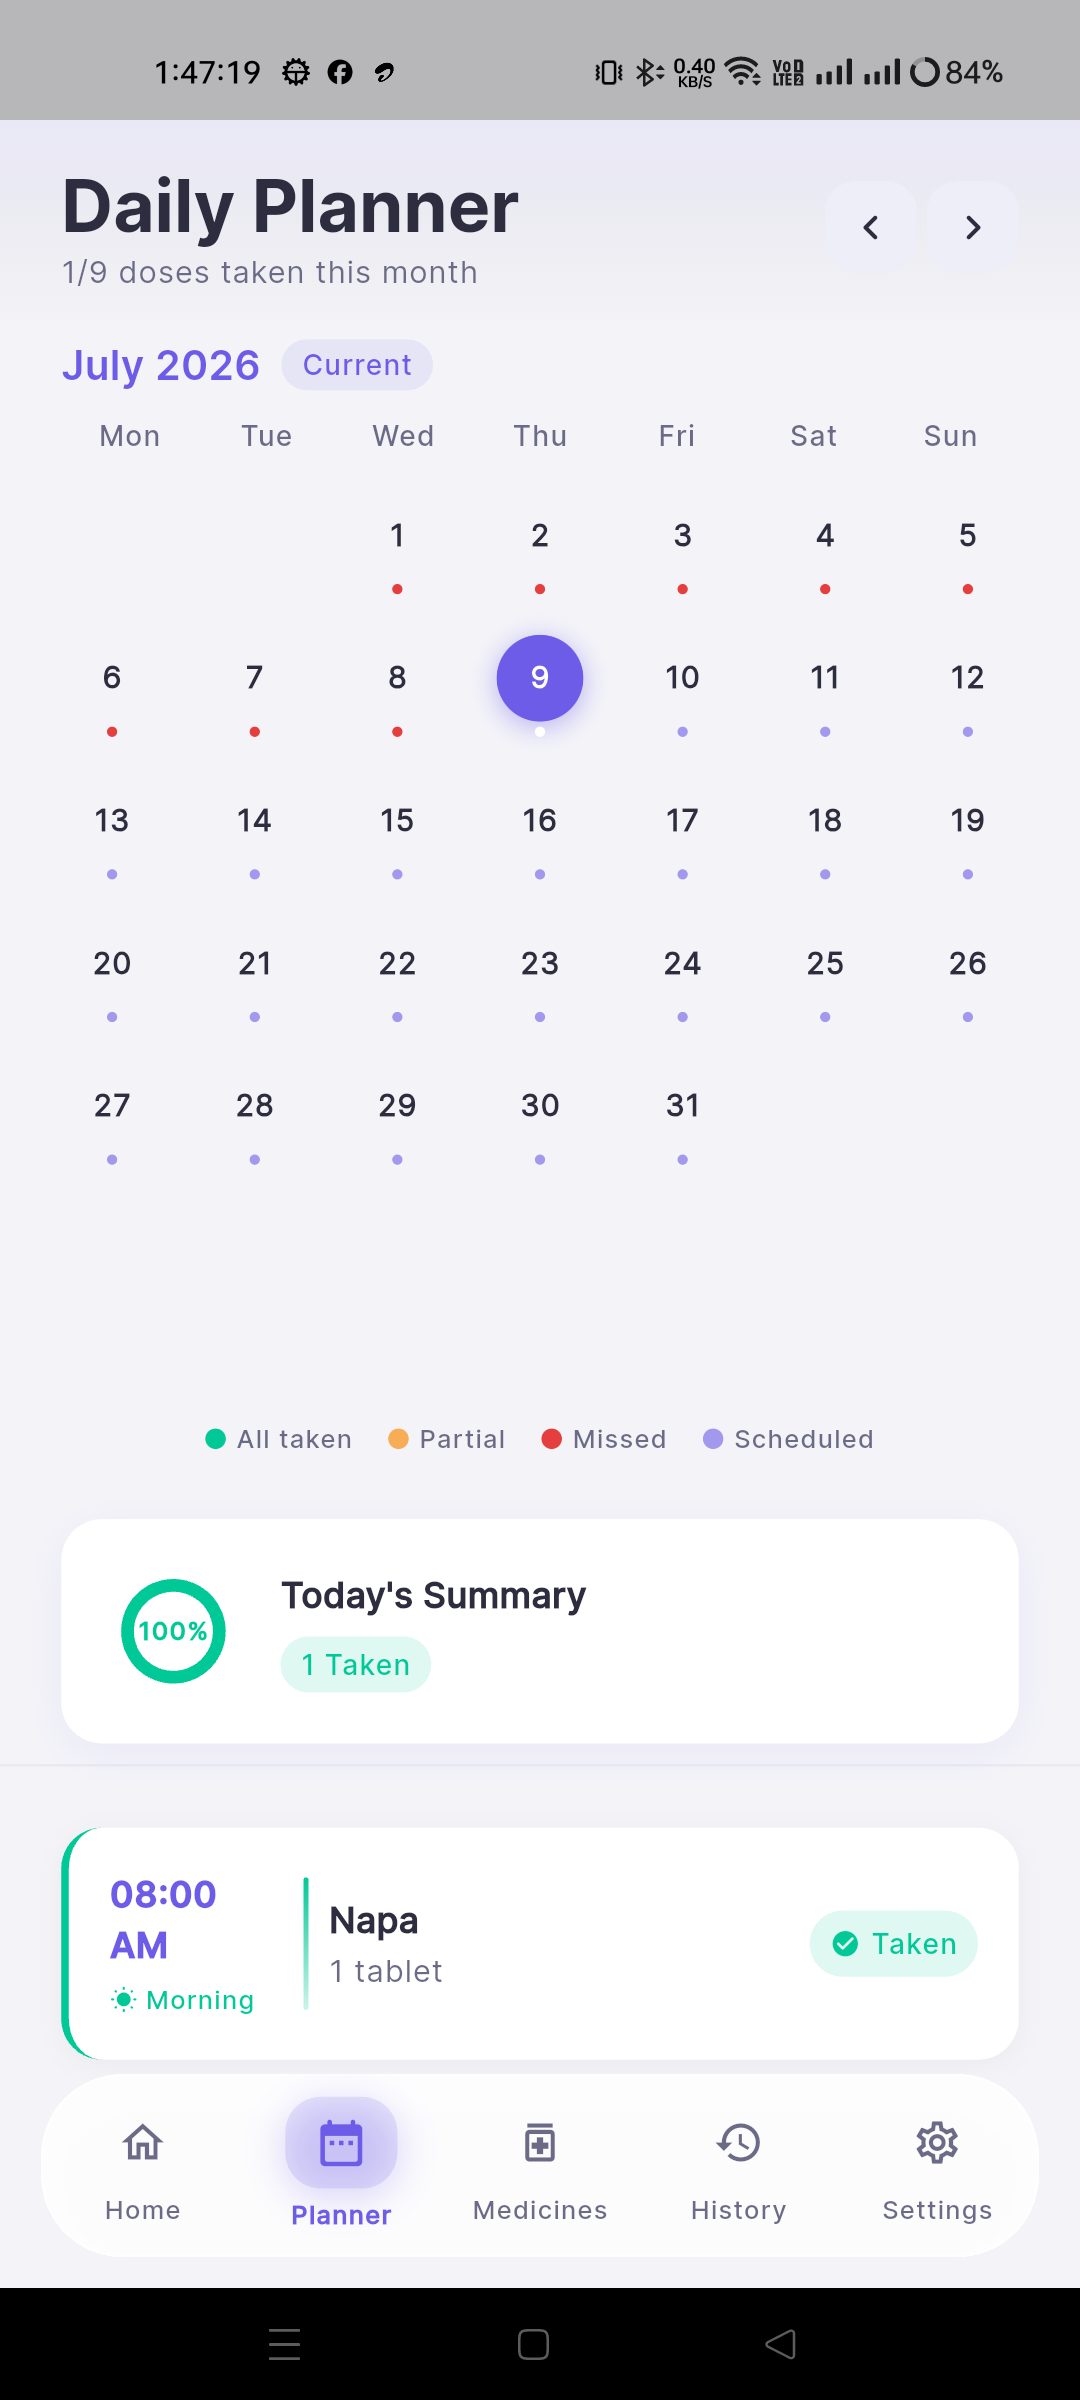
\includegraphics[width=0.5\textwidth]{screenshots/18_daily_planner.png}
    \caption{Daily Planner with adherence heatmap}
\end{figure}

% ─────────────────────────────────────────────────────────────
\section{History}

The \textbf{History} tab summarizes your adherence over time: a "this week"
percentage with taken/missed/skipped counts, a monthly adherence heatmap
(same colour legend as the Planner), and a chronological \textbf{Dose log}
listing every recorded dose event.

\begin{figure}[H]
    \centering
    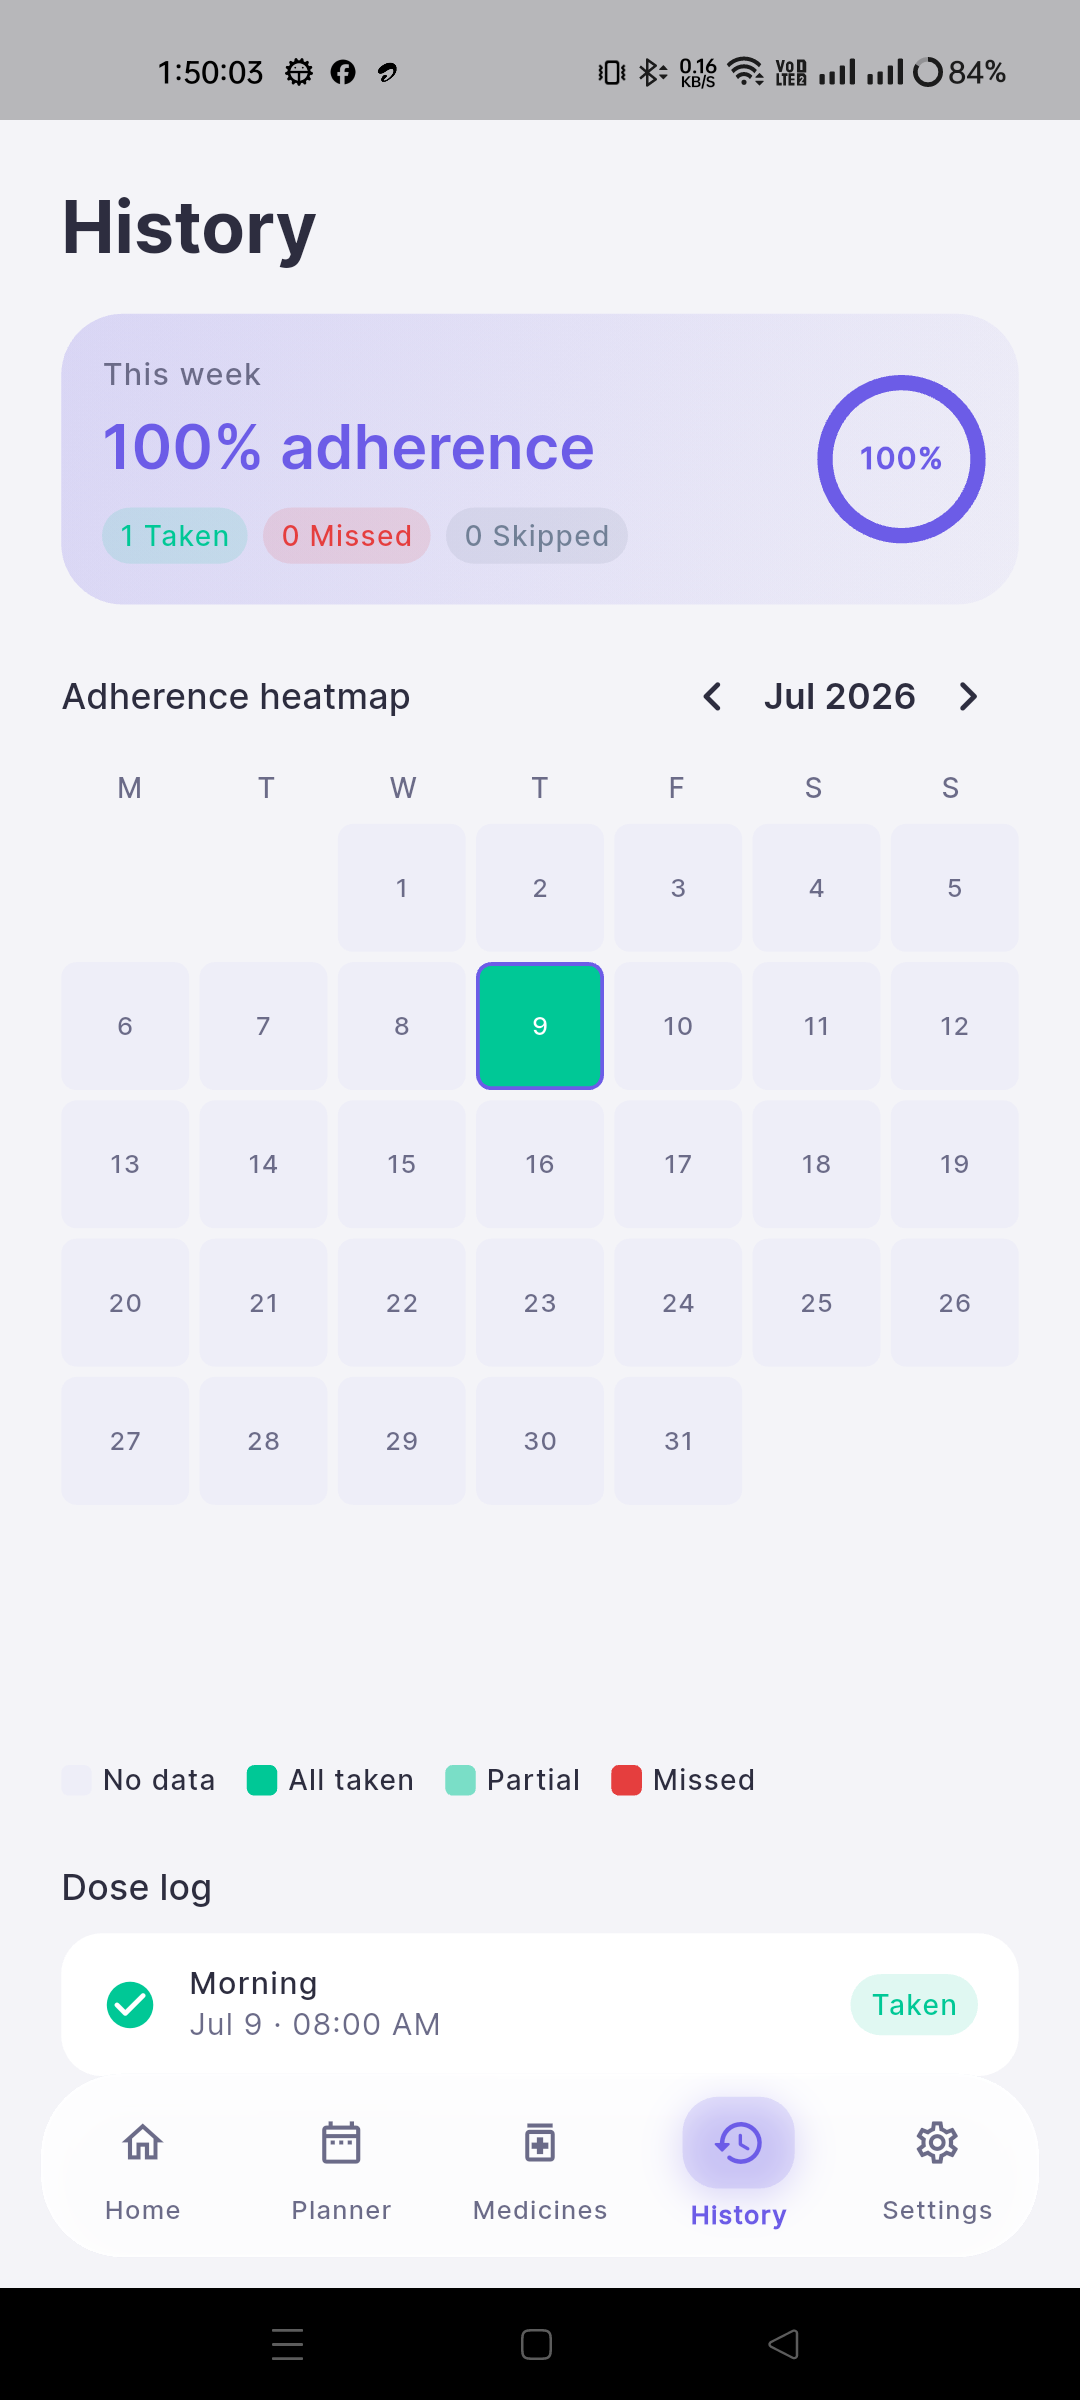
\includegraphics[width=0.5\textwidth]{screenshots/19_history.png}
    \caption{History — adherence heatmap and dose log}
\end{figure}

% ─────────────────────────────────────────────────────────────
\section{Settings}

The \textbf{Settings} tab holds your profile and app preferences.

\begin{figure}[H]
    \centering
    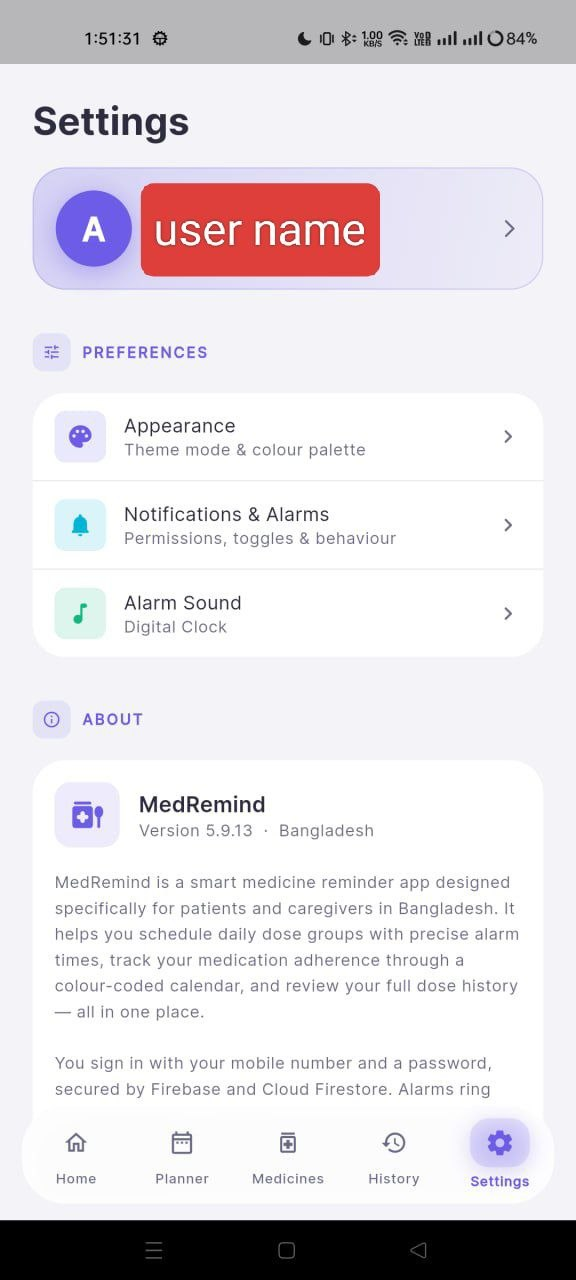
\includegraphics[width=0.45\textwidth]{screenshots/20_settings.jpg}
    \caption{Settings — profile, preferences, and about}
\end{figure}

\subsection{Preferences}
\begin{itemize}[leftmargin=1.5em]
    \item \textbf{Appearance} — theme mode and colour palette.
    \item \textbf{Notifications \& Alarms} — permissions, toggles, and
        behaviour for how reminders fire.
    \item \textbf{Alarm Sound} — choose the ringtone used for the
        full-screen alarm.
\end{itemize}

\subsection{My Profile}

Tapping your name at the top of Settings opens your profile, showing your
mobile number and subscription status/expiry, plus account actions:

\begin{itemize}[leftmargin=1.5em]
    \item \textbf{Logout} — sign out of this device only; your account and
        data remain.
    \item \textbf{Change Password} — update your password (requires your
        current one).
    \item \textbf{Unsubscribe} — cancels your BDApps subscription
        \emph{and} permanently deletes your account and all its data. This
        cannot be undone.
\end{itemize}

\begin{figure}[H]
    \centering
    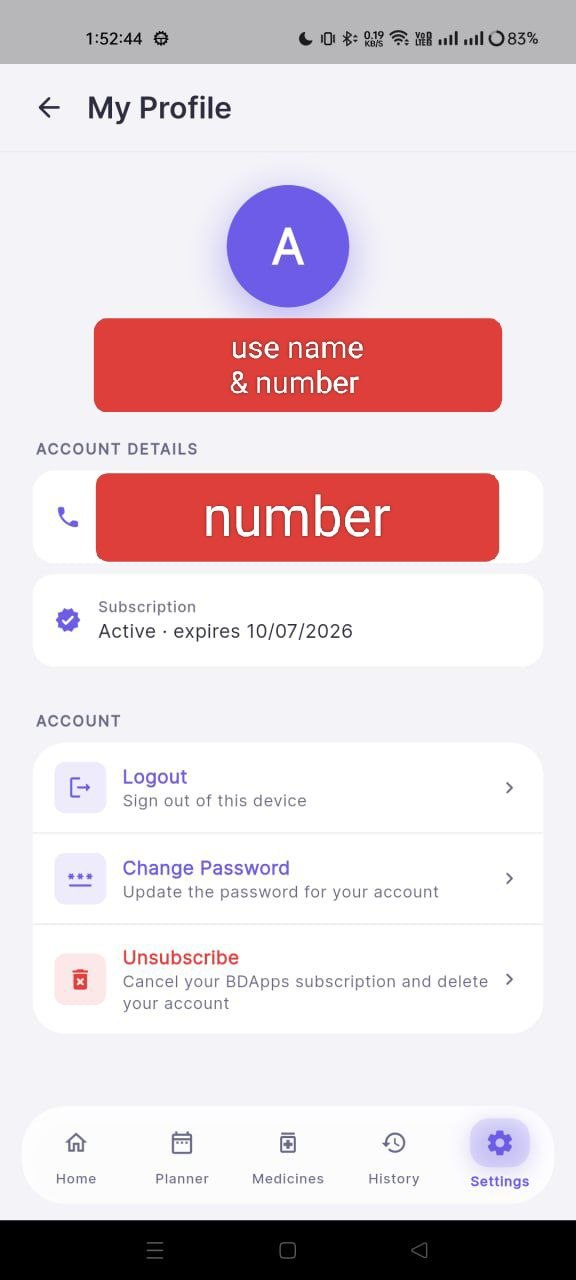
\includegraphics[width=0.45\textwidth]{screenshots/21_profile.jpg}
    \caption{My Profile — account details and account actions}
\end{figure}

% ─────────────────────────────────────────────────────────────
\section{Tips for Reliable Reminders}

\begin{enumerate}[leftmargin=1.5em]
    \item Grant \textbf{Exact Alarms} and disable \textbf{Battery
        Optimization} for MedRemind when prompted — without these, some
        Android phones delay or silently drop alarms.
    \item Keep the app installed and signed in; alarms are scheduled locally
        on your device and don't need an active internet connection to ring.
    \item Use \textbf{Dose Groups} rather than one-off reminders — grouping
        medicines by time keeps the Home screen and Planner clean and
        accurate.
    \item Check the \textbf{History} tab periodically; a string of missed or
        skipped doses is worth discussing with your doctor or caregiver.
\end{enumerate}

\end{document}
